\documentclass[11pt,a4paper]{article}
\usepackage[T1]{fontenc}
\usepackage[utf8]{inputenc}
\usepackage[english]{babel}
\usepackage{newtxtext,newtxmath}
\usepackage[scaled=0.93]{helvet}
\usepackage[a4paper,top=23mm,bottom=24mm,left=24mm,right=24mm,headheight=15pt]{geometry}
\usepackage{microtype,graphicx,booktabs,tabularx,longtable,array}
\usepackage[table]{xcolor}
\usepackage{caption,subcaption,enumitem,fancyhdr,lastpage,float,placeins}
\usepackage{tikz}
\usetikzlibrary{arrows.meta,positioning,fit,backgrounds,calc,shapes.geometric}
\usepackage{titlesec,listings,xurl}
\usepackage[hidelinks,pdfusetitle]{hyperref}
\definecolor{ink}{HTML}{16334A}
\definecolor{accent}{HTML}{087E83}
\definecolor{light}{HTML}{F0F4F6}
\definecolor{muted}{HTML}{536573}
\definecolor{warning}{HTML}{AC6518}
\hypersetup{pdftitle={IndiCare Mobile IoT Monitoring Technical Report},pdfauthor={IndiCare project},pdfsubject={IOT308TC Assessment 2 evidence based technical report}}
\graphicspath{{figures/}}
\setlength{\parindent}{0pt}
\setlength{\parskip}{5.5pt plus 1pt}
\setlength{\emergencystretch}{2em}
\renewcommand{\arraystretch}{1.18}
\newcolumntype{Y}{>{\raggedright\arraybackslash}X}
\newcolumntype{P}[1]{>{\raggedright\arraybackslash}p{#1}}
\captionsetup{font=small,labelfont=bf,labelsep=period,skip=7pt}
\captionsetup[subfigure]{font=small,labelfont=bf}
\titleformat{\section}{\large\sffamily\bfseries}{\thesection}{0.7em}{}
\titleformat{\subsection}{\normalsize\sffamily\bfseries}{\thesubsection}{0.7em}{}
\titlespacing*{\section}{0pt}{16pt}{7pt}
\titlespacing*{\subsection}{0pt}{10pt}{4pt}
\setlist{nosep,leftmargin=1.5em,topsep=5pt}
\setcounter{tocdepth}{1}
\setcounter{topnumber}{3}
\setcounter{bottomnumber}{2}
\renewcommand{\topfraction}{0.92}
\renewcommand{\bottomfraction}{0.8}
\renewcommand{\textfraction}{0.07}
\renewcommand{\floatpagefraction}{0.78}
\pagestyle{fancy}
\fancyhf{}
\fancyhead[L]{\small\sffamily IndiCare}
\fancyhead[R]{\small\sffamily IOT308TC Assessment 2}
\fancyfoot[L]{\footnotesize Educational prototype}
\fancyfoot[R]{\footnotesize\thepage}
\renewcommand{\headrulewidth}{0.3pt}
\newenvironment{reportprose}{}{}
\newcommand{\code}[1]{\texttt{\detokenize{#1}}}
\newcommand{\evidencebox}[2]{\begin{quote}\small\textbf{#1}\par #2\end{quote}}
\lstset{basicstyle=\small\ttfamily,breaklines=true,columns=fullflexible,keepspaces=true,frame=single,rulecolor=\color{muted},backgroundcolor=\color{light},aboveskip=8pt,belowskip=8pt}
% Team information supplied by the project members.
\newcommand{\ReportMembers}{%
\begin{tabular}[t]{@{}l@{\hspace{7mm}}l@{}}
Nathan Ratichon & 2362789\\
Guannan Ge & 2364229\\
Jose Manuel Cortes Ceron & 2686162\\
Cheng Zhang & 2361292
\end{tabular}}
\newcommand{\ReportTutor}{Matilda Isaac}
\newcommand{\ReportDate}{31 October 2026}
\newcommand{\ReportRepository}{https://github.com/deepdevjose/Older-Monitoring-Wearable}

% Current revision facts. Update from executed release records, never estimates.
% Historical evidence files remain dated baseline snapshots.
\newcommand{\CurrentRevisionDate}{29 October 2026}
\newcommand{\CurrentVersionCode}{19}
\newcommand{\CurrentPythonResult}{229/229 tests}
\newcommand{\CurrentJvmResult}{3,240 assertions}
\newcommand{\CurrentHistoryResult}{22 tests passed}
\newcommand{\CurrentLearningResult}{14 tests passed}
\newcommand{\CurrentAndroidResult}{Code 19 installed on SM-S901E / Android 13: 878 native onboarding and layout checks. Separately, 7,273 isolated preview checks and 48 captures exercise both roles at 100\%/200\% text using production Java/resources and fictional state. No current Bluetooth or server delivery claim}
\newcommand{\CurrentAndroidTableResult}{878 native checks; 7,273 isolated preview checks and 48 captures at 100\%/200\% text. Installed S22 / Android 13; fixtures do not establish physical delivery}
\newcommand{\CurrentIntegrationResult}{24/24 checks}
\newcommand{\CurrentApkHash}{afdc41baa3938caab845839f5f636e4960f08f3921f125559e6f8e6d6425ba2a}

\newcommand{\USBCaptureRecords}{76}
\newcommand{\USBRecordId}{300}
\newcommand{\USBSampleId}{ffb53673-c98c-435e-81ed-00ef2d9bd3f5}
\newcommand{\USBRecordTimestamp}{2026-10-30T18:09:13.093000Z}

\newcommand{\MainWordCount}{3,215}

% Vector figures for the evidence-led IndiCare report.
% Shared palette/styles and system views are provided by diagram_system.tex.
% Source-audited deployment, component, class, data and security maps.
% Shared palette/geometry lives in diagram_styles.tex. Units: cm.
\newcommand{\ArchitectureDiagram}{%
\begin{figure}[H]\centering
\begin{tikzpicture}
% Three physical responsibilities; colour separates runtime from offline work.
\path[fill=bluewash,rounded corners=3pt] (11.5,.85) rectangle (15.6,-8.35);
\node[dHeading,anchor=west] at (11.75,.55) {SELF-HOSTED PC};
\node[dBox,text width=2.8cm,minimum height=3.25cm] (wearable) at (1.6,-1.5)
 {\textbf{01 / Wearable}\\[4pt]KEYES + ESP32\\MAX30102 / GY906\\MPU6050\\[4pt]Acquire + flag validity\\Buzzer output: GPIO25};
% Phone silhouette remains legible without using a mock screenshot.
\draw[draw=accent,fill=white,line width=.85pt,rounded corners=6pt] (5.25,.25) rectangle (8.75,-3.25);
\draw[stroke,line width=1.3pt,line cap=round] (6.55,.07)--(7.45,.07);
\node[dNote,text=ink,text width=2.95cm,anchor=north west] at (5.52,-.2)
 {\textbf{02 / Adult Android app}\\[5pt]CareMonitor\\Authenticate wearable\\Encrypt upload queue\\Readings + history\\Saved Learning insights};
\coordinate (phoneIn) at (5.25,-1.35);\coordinate (phoneOut) at (8.75,-1.35);
\node[dBox,text width=2.9cm,minimum height=2.65cm] (api) at (13.55,-1.65)
 {\textbf{03 / FastAPI}\\[4pt]REST JSON /api/v1\\Roles + approved links\\Readings / history / inbox\\SQLite + encrypted fields};
\draw[dFlow] (wearable.east|-phoneIn)--(phoneIn);
\draw[dReturn] (5.25,-1.85)--(3.22,-1.85);
\node[dLabel,text width=1.8cm] at (4.23,-.6) {Classic SPP\\NDJSON telemetry};
\node[dLabel,text width=1.8cm] at (4.23,-2.55) {CM1 mutual\\authentication};
\draw[dFlow] (phoneOut)--(api.west|-phoneOut);
\draw[dReturn] (api.west|-0,-1.85)--(8.75,-1.85);
\node[dLabel,text width=2.1cm] at (10.15,-.65) {HTTPS / TLS\\REST JSON + token};
\node[dLabel,text width=2.1cm] at (10.15,-2.55) {Upload / query\\Parsed response};
% Caregiver has a real connection, rather than an unconnected paragraph.
\node[dData,text width=2.8cm,minimum height=1.6cm] (care) at (1.6,-4.7)
 {\textbf{04 / Caregiver app}\\Approved adult selection\\History + private notices};
\draw[draw=accent,line width=.85pt,{Stealth[length=2mm]}-{Stealth[length=2mm]}]
 (care.east)--(10.9,-4.7)--(10.9,-3.05)--(api.south west);
\node[dLabel,text width=5.7cm] at (7.1,-4.2) {HTTPS long polling and authorised GET\\Adult approval controls the shared resource};
% Independent training is separate from deployed native inference.
\node[dBox,fill=light,text width=2.8cm,minimum height=1.7cm] (csv) at (1.6,-7.25)
 {\textbf{Synthetic dataset}\\Grouped row split\\Educational labels};
\node[dBox,fill=light,text width=3cm,minimum height=1.7cm] (train) at (7,-7.25)
 {\textbf{Offline model comparison}\\Logistic Regression / RF\\Select on validation};
\node[dData,text width=2.9cm,minimum height=1.7cm] (model) at (13.55,-7.25)
 {\textbf{Loaded health model}\\Hash + version checks\\Class + confidence score};
\draw[dReturn] (csv)--node[dLabel,above]{Train / evaluate}(train);
\draw[dReturn] (train)--node[dLabel,above]{Saved artefact}(model);
\draw[dFlow] (api.south)--node[dLabel,right,text width=1.9cm]{Synthetic-only\\Learning API}(model.north);
\node[dNote,anchor=west] at (.05,-9.05) {\textbf{Legend}\quad Solid: implemented runtime communication.\quad Dashed: reply or offline artefact path, as labelled.};
\end{tikzpicture}
\caption{Complete system and its separate care and synthetic-learning paths. Physical SPP, API-backed native views and saved synthetic confidence were exercised in the controlled code-22 screen campaign; model training was evaluated independently. USB forwarding carried HTTPS in that campaign; reachable LAN deployment uses the same API. The two roles were exercised successively on one S22.}\label{fig:architecture}
\end{figure}}

\newcommand{\ProtocolStackFigure}{%
\begin{table}[H]\centering\small
\caption{Implemented communication boundaries. Cryptographic controls and local persistence are distinguished from transport protocols.}\label{tab:protocol-stack}
\begin{tabularx}{\textwidth}{@{}P{28mm}P{47mm}Y@{}}\toprule
Boundary & Protocol / format & Contract and protection\\\midrule
Sensors / ESP32 & I\textsuperscript{2}C / SMBus, 100 kHz & GPIO21 SDA, GPIO22 SCL; 7-bit addresses 0x57 / 0x5A / 0x68. Common ground and compatible logic.\\
ESP32 / phone & Classic Bluetooth SPP; RFCOMM UUID 0x1101; UTF-8 NDJSON & Encrypted link plus CM1 HMAC-SHA256 proofs. One active phone; telemetry after CM1 READY. This firmware does not expose BLE GATT.\\
Phone / PC carrier & USB adb reverse, or LAN IP/TCP & USB maps phone loopback to PC loopback. LAN normally uses port 8443. Both carry the same certificate-verified HTTPS application traffic.\\
App / FastAPI & HTTPS REST JSON, /api/v1 & Certificate chain and hostname checks; Bearer token; per-resource role and approved-link authorisation.\\
Private care inbox & Authenticated HTTPS long polling & Incremental durable inbox IDs. Delivery acknowledgement, human review and episode recovery are separate operations.\\
Services / SQLite & sqlite3 transactions and WAL & Unique sample IDs, atomic fanout and encrypted sensitive fields. AES-GCM is field protection, not full-file database encryption.\\
Optional board clock & Wi-Fi / IP / UDP / NTP & Time synchronisation requires reachability. Missing wearable timestamps use phone receipt time; NTP does not authenticate measurements.\\\bottomrule
\end{tabularx}
\end{table}}

\newcommand{\ServerArchitectureDiagram}{%
\begin{figure}[H]\centering
\begin{tikzpicture}
\node[dBox,fill=bluewash,text width=14.6cm,minimum height=1.15cm] (entry) at (7.55,0)
 {\textbf{HTTPS boundary / Uvicorn + FastAPI}\\Request limits $\rightarrow$ closed Pydantic schemas $\rightarrow$ session lookup $\rightarrow$ resource authorisation};
\node[dBox,text width=4.1cm,minimum height=2.1cm] (care) at (2.3,-2.3)
 {\textbf{Care resources}\\[4pt]Accounts / approved links\\Readings / overview / history\\Consent / events / reminders};
\node[dBox,text width=4.1cm,minimum height=2.1cm] (rules) at (7.55,-2.3)
 {\textbf{Episodes + private inbox}\\[4pt]Source-scoped limit rules\\Persistent alert / recovery\\Per-user delivery + review};
\node[dData,text width=4.1cm,minimum height=2.1cm] (ml) at (12.8,-2.3)
 {\textbf{Synthetic learning}\\[4pt]Classify + save exercises\\Model hash/version check\\Separate SisFall experiment};
\draw[dFlow] (entry.south)--(7.55,-.95)-|(care.north);
\draw[dFlow] (7.55,-.95)--(rules.north);
\draw[dFlow] (7.55,-.95)-|(ml.north);
\node[dBox,fill=light,text width=14.6cm,minimum height=1.25cm] (vault) at (7.55,-4.95)
 {\textbf{Database + Vault / transaction boundary}\\Commit readings and eligible side effects together; unique sample identity protects retries.\\Device diagnostics, synthetic rule input and saved model exercises retain distinct provenance.};
\foreach \n in {care,rules,ml} \draw[dFlow] (\n.south)--(\n.south|-0,-3.85)--(7.55,-3.85)--(vault.north);
\node[dData,text width=14.6cm,minimum height=1.05cm] (db) at (7.55,-6.85)
 {\textbf{SQLite on the self-hosted PC}\\WAL / synchronous FULL / foreign keys; selected sensitive fields protected with AES-256-GCM};
\draw[dFlow] (vault)--(db);
\end{tikzpicture}
\caption{Server runtime responsibilities. Arrows show request/service dependencies and persistence, rather than a single diagnostic pipeline. Physical wearable envelopes are stored as diagnostics; the synthetic model does not classify surface-temperature measurements as core body temperature.}\label{fig:server-architecture}
\end{figure}}

\newcommand{\ServerClassDiagram}{%
\begin{figure}[H]\centering
\begin{tikzpicture}[
 cls/.style={dBox,text width=4.2cm,minimum height=1.8cm},
 dep/.style={dReturn},inherit/.style={-{Triangle[open,length=2.2mm,width=2.4mm]},draw=accent,line width=.85pt}]
\node[cls] (settings) at (2.3,0) {\textbf{Settings}\quad config.py\\[3pt]data\_dir / session\_hours\\load\_key() / initialize\_key()};
\node[cls,fill=bluewash] (database) at (7.55,0) {\textbf{Database}\quad db.py\\[3pt]connect() / transaction()\\audit() / rate\_limit()};
\node[cls] (vault) at (12.8,0) {\textbf{Vault}\quad security.py\\[3pt]seal() / open() / lookup()\\AES-GCM / keyed lookups};
\draw[dep] (database)--(settings);\draw[dep] (database)--(vault);
\node[cls] (schemas) at (2.3,-3.1) {\textbf{ClosedModel}\quad schemas.py\\[3pt]Pydantic BaseModel\\Register / Reading / Event};
\node[cls,fill=bluewash] (api) at (7.55,-3.1) {\textbf{FastAPI route functions}\\[3pt]Session + patient guards\\RequestSecurity middleware};
\node[cls] (health) at (12.8,-3.1) {\textbf{ModelService}\quad ml.py\\[3pt]predict(features, source)\\Saved health-model artefact};
\draw[dep] (api)--(database);\draw[dep] (api)--(schemas);\draw[dep] (api)--(health);
\node[cls] (classification) at (2.3,-6.2) {\textbf{ClassificationRequest}\\routes\_ml.py\\[3pt]Synthetic features + freshness};
\node[cls,fill=bluewash] (services) at (7.55,-6.2) {\textbf{Service modules}\\[3pt]alerts / history / push\\Eligible episodes / rollups / inbox};
\node[cls] (fall) at (12.8,-6.2) {\textbf{FallModelService}\\fall\_ml.py\\[3pt]Independent SisFall model};
\draw[dep] (api)--(services);
\draw[dep] (api.east)--(10.1,-3.1)--(10.1,-4.65)-|(fall.north);
\node[cls] (learning) at (2.3,-9.1) {\textbf{LearningReading}\quad learning.py\\[3pt]sample\_id: UUID};
\draw[inherit] (learning)--(classification);
\node[dNote,text width=9.1cm,anchor=north west] at (5.4,-8.5)
 {\textbf{Legend}\quad Dashed: uses/dependency. Hollow triangle: inheritance.\\[5pt]
  LearningReading extends ClassificationRequest; it does not directly extend ClosedModel. Routes and module functions are shown as functions, not invented controller classes.};
\end{tikzpicture}
\caption{Selected server types and dependencies, derived from the named Python modules. The separate SisFall service remains an experimental model endpoint; it is not a live MPU6050-to-fall alarm pipeline.}\label{fig:server-classes}
\end{figure}}

\newcommand{\DatabaseDiagram}{%
\begin{figure}[H]\centering
\begin{tikzpicture}[
 entity/.style={dBox,text width=3.75cm,minimum height=1.8cm},
 relation/.style={draw=accent,line width=.75pt},
 cardinal/.style={font=\sffamily\fontsize{7.5}{9}\selectfont,text=muted,fill=white,inner sep=1.5pt}]
\node[entity,fill=bluewash] (users) at (2.1,0) {\textbf{users}\\PK id / role\\Encrypted profile\\Argon2id password hash};
\node[entity,fill=bluewash] (patients) at (7.55,0) {\textbf{patients}\\PK/FK id $\rightarrow$ users\\One adult resource};
\node[entity,fill=bluewash] (members) at (13,0) {\textbf{memberships}\\PK elder\_id + caregiver\_id\\Approved adult / caregiver link};
\draw[relation] (users)--node[cardinal,near start,above]{1}node[cardinal,near end,above]{0..1}(patients);
\draw[relation] (patients)--node[cardinal,near start,above]{1}node[cardinal,near end,above]{*}(members);
\draw[relation] (members.north)--(13,1.5)--(2.1,1.5)--(users.north);
\node[cardinal] at (7.55,1.5) {Each membership references 1 caregiver user; a caregiver may hold * memberships};
\node[entity] (sessions) at (2.1,-3.2) {\textbf{sessions + notifications}\\FK user\_id\\Token hash / private inbox\\Expiry / delivery state};
\node[entity] (readings) at (7.55,-3.2) {\textbf{readings + rollups}\\FK elder\_id\\Unique adult/sample identity\\Source + encrypted envelope};
\node[entity] (alerts) at (13,-3.2) {\textbf{alerts + rule state}\\FK elder\_id\\Persistent episode pointer\\Recovery + per-user review};
\draw[relation] (users)--node[cardinal,left]{1 : *}(sessions);
\draw[relation] (patients)--node[cardinal,right]{1 : *}(readings);
\fill[accent] (7.55,-1.5) circle (1pt);
\draw[relation] (7.55,-1.5)--(10.25,-1.5)--(10.25,-3.2)--node[cardinal,above]{1 : *}(alerts.west);
\node[entity] (privacy) at (2.1,-6.5) {\textbf{consents + locations}\\Adult-owned settings\\0..1 consent row per adult\\* expiring location records};
\node[entity] (learning) at (7.55,-6.5) {\textbf{learning\_records}\\FK elder\_id\\Unique adult/sample identity\\Encrypted synthetic exercises};
\node[entity] (care) at (13,-6.5) {\textbf{care + approval records}\\Reminders / occurrences\\Invitations / link requests\\Events / source metadata};
\draw[relation] (7.55,-1.5)--(4.85,-1.5)--(4.85,-5)--(2.1,-5)--(privacy.north);
\draw[relation] (10.25,-3.2)--(10.25,-5.2)--(13,-5.2)--node[cardinal,right]{1 : *}(care.north);
\fill[accent] (10.25,-3.2) circle (1pt);
\draw[relation] (10.25,-5.2)--(7.55,-5.2)--node[cardinal,right]{1 : *}(learning.north);
\fill[accent] (10.25,-5.2) circle (1pt);
\node[dNote,text width=15.1cm,anchor=north west] at (0,-8.05)
 {Grouped ownership map, not the full physical ERD. Patient-owned groups use elder\_id; notifications also reference an adult resource. alert\_acknowledgements uses (alert\_id, user\_id). Operational tables audit and rate\_limits are omitted for clarity.};
\end{tikzpicture}
\caption{Principal SQLite ownership relationships from db.py. Cardinalities describe the database contracts, while grouped records retain their own keys and constraints. Selected fields are encrypted; indexed identifiers and timestamps remain visible metadata.}\label{fig:database-domains}
\end{figure}}

\newcommand{\SecurityProtocolDiagram}{%
\begin{figure}[H]\centering
\begin{tikzpicture}
\node[dHeading,anchor=west] at (0,.65) {Independent trust boundaries};
\node[dBox,fill=bluewash,text width=4.15cm,minimum height=.7cm] at (2.3,0) {\textbf{01 / Account and API}};
\node[dBox,fill=tealwash,text width=4.15cm,minimum height=.7cm] at (7.55,0) {\textbf{02 / Wearable link}};
\node[dBox,fill=bluewash,text width=4.15cm,minimum height=.7cm] at (12.8,0) {\textbf{03 / Private persistence}};
\node[dBox,text width=4.15cm,minimum height=3.8cm,anchor=north] at (2.3,-.8)
 {\textbf{HTTPS + authorisation}\\[6pt]Certificate and host checks\\Argon2id: t=3 / m=64 MiB / p=2\\48 random token bytes\\SHA-256 token hashes\\[6pt]Role + approved relationship\\Expiry and revocation};
\node[dBox,text width=4.15cm,minimum height=3.8cm,anchor=north] at (7.55,-.8)
 {\textbf{SPP + CM1 key possession}\\[6pt]Encrypted Classic Bluetooth\\Private 128-bit board key\\Fresh 128-bit nonces\\HMAC-SHA256 proofs\\[6pt]HELLO / CHALLENGE\\AUTH / READY\\10 s handshake deadline};
\node[dBox,text width=4.15cm,minimum height=3.8cm,anchor=north] at (12.8,-.8)
 {\textbf{Authenticated field storage}\\[6pt]AndroidKeyStore + AES-GCM\\Server Vault: AES-256-GCM\\96-bit random nonce\\Record-bound associated data\\[6pt]Unique sample ID + digest\\Commit before upload ACK};
\node[dData,text width=14.6cm,minimum height=.95cm] at (7.55,-5.65)
 {\textbf{Actual setup order}\quad Adult sign-in $\rightarrow$ private wearable-key setup $\rightarrow$ SPP link and CM1 authentication $\rightarrow$ sensor JSON.\\The columns above group controls; they do not represent a single sequential login protocol.};
\node[dNote,text width=14.8cm,anchor=north west] at (.1,-6.65)
 {Pairing without board input is not proof of resistance to an active pairing relay. Field encryption does not hide SQLite metadata. No passwords, bearer tokens, board keys or proof values appear in the report.};
\end{tikzpicture}
\caption{Implemented security controls across account, radio and storage boundaries. Session authorisation remains independent of Bluetooth key possession. One active phone owns the SPP link; telemetry follows successful CM1 authentication.}\label{fig:security-boundaries}
\end{figure}}


\newcommand{\SequenceDiagram}{%
\begin{figure}[H]\centering
\begin{tikzpicture}[
 font=\sffamily\fontsize{8.5}{11}\selectfont,
 participant/.style={dBox,fill=bluewash,text width=2.35cm,minimum height=.85cm,align=center,inner sep=4pt},
 request/.style={-{Stealth[length=1.7mm]},draw=accent,line width=.8pt},
 reply/.style={-{Stealth[length=1.7mm]},draw=muted,dashed,line width=.65pt},
 msg/.style={dLabel,font=\sffamily\fontsize{8}{10}\selectfont,align=center,fill=white,inner sep=2pt}]
\node[participant] (sender) at (0,0) {\textbf{Sender}\\Synthetic envelope};
\node[participant] (api) at (3.3,0) {\textbf{FastAPI}\\Auth + validation};
\node[participant] (store) at (6.6,0) {\textbf{SQLite}\\Atomic services};
\node[participant] (c1) at (9.9,0) {\textbf{Caregiver A}\\Private inbox};
\node[participant] (c2) at (13.2,0) {\textbf{Caregiver B}\\Private inbox};
\foreach \n in {sender,api,store,c1,c2}
 \draw[stroke,densely dashed,line width=.55pt] (\n.south)--(\n.south|-0,-12.45);
\draw[request] (0,-1.50)--node[msg,above]{POST /readings\\new sample\_id}(3.3,-1.50);
\draw[request] (3.3,-2.30)--node[msg,above]{Check unique key + digest\\Insert encrypted reading}(6.6,-2.30);
\draw[request] (6.6,-2.95)--(7.25,-2.95)--(7.25,-3.60)--(6.6,-3.60);
\node[msg,text width=5.3cm,anchor=west] at (7.7,-3.25)
 {Third eligible abnormal sample:\\one episode; adult, A and B inbox entries};
\draw[reply] (6.6,-4.25)--node[msg,above]{COMMIT; record ID}(3.3,-4.25);
\draw[reply] (3.3,-5.05)--node[msg,above]{201 response lost\\Retry scenario}(0,-5.05);
\draw[request] (0,-5.85)--node[msg,above]{Retry identical envelope\\Same sample\_id}(3.3,-5.85);
\draw[request] (3.3,-6.65)--node[msg,above]{Existing key + identical digest}(6.6,-6.65);
\draw[reply] (6.6,-7.45)--node[msg,above]{Same record; no new alert or fanout}(3.3,-7.45);
\draw[reply] (3.3,-8.25)--node[msg,above]{201; duplicate: true}(0,-8.25);
\draw[request] (9.9,-9.05)--node[msg,above,pos=.48]{A: authenticated long poll}(3.3,-9.05);
\draw[reply] (3.3,-9.85)--node[msg,above,pos=.48]{A's durable inbox item}(9.9,-9.85);
\draw[request] (13.2,-10.65)--node[msg,above,pos=.55]{B: independent authenticated long poll}(3.3,-10.65);
\draw[reply] (3.3,-11.45)--node[msg,above,pos=.55]{B's durable inbox item}(13.2,-11.45);
\draw[request] (9.9,-12.25)--node[msg,above,pos=.48]{A reviews: per-user acknowledgement}(3.3,-12.25);
\node[dNote,text width=14.4cm,anchor=north] at (6.6,-12.85)
 {\tikz{\draw[request](0,0)--(.55,0);}\quad Request / operation\qquad
 \tikz{\draw[reply](0,0)--(.55,0);}\quad Response\\[3pt]
 Changed content with the same sample ID returns 409. Delivery acknowledgement, caregiver review and episode recovery are independent.};
\end{tikzpicture}
\caption{Atomic reception, safe retry and independent recipient fanout. The reading, any eligible rule episode and recipient inbox entries commit together; an identical retry returns the existing record. This contract was verified with loopback clients; simultaneous delivery to two physical phones is not claimed.}\label{fig:sequence}
\end{figure}}

\newcommand{\AlertStateDiagram}{%
\begin{figure}[H]\centering
\begin{tikzpicture}[font=\sffamily\fontsize{8.5}{11}\selectfont,
 state/.style={dBox,text width=3.65cm,minimum height=1.5cm,align=center},
 transition/.style={dFlow},
 edge label/.style={dLabel,font=\sffamily\fontsize{8}{10}\selectfont,align=center,text width=1.25cm}]
\node[state] (idle) at (2.2,0)
 {\textbf{No active episode}\\No active alert pointer\\Per patient and rule};
\node[state,fill=tealwash,draw=teal] (open) at (7.6,0)
 {\textbf{Open episode}\\One persistent alert ID\\Duplicates suppressed};
\node[state] (recovered) at (13,0)
 {\textbf{Recovered episode}\\recovered\_at recorded\\Active pointer cleared};
\draw[transition] (idle.east)--node[edge label,above]{3 present\\abnormal\\estimates}(open.west);
\draw[transition] (open.east)--node[edge label,above]{3 present\\normal\\estimates}(recovered.west);
\draw[transition] (recovered.north)--(13,1.7)--node[dLabel,above]{New three-sample trigger creates a new alert ID}(7.6,1.7)--(open.north);
\draw[transition] (open.south)--(7.6,-1.55)--(5,-1.55)--(5,-.75)--(open.south west);
\node[dLabel,text width=4.8cm,align=center,anchor=north] at (4.65,-1.9)
 {Continued trigger or ineligible input:\\keep the current episode open};
\node[dBox,fill=bluewash,text width=5.4cm,minimum height=1.3cm] (review) at (12.1,-2.5)
 {\textbf{Independent caregiver review}\\Record (alert\_id, user\_id)\\Review does not close or recover an episode};
\draw[dReturn] (open.south east)--(9.65,-1.25)-|(review.north);
\node[dNote,text width=14.5cm,anchor=north] at (7.6,-3.65)
 {\textbf{Eligibility gate:} the latest three readings must share patient and source, be fresh within two minutes, correctly ordered and 1--30 seconds apart. Optical rules use present numerical estimates with contact; quality metadata is retained. Missing contact, stale data or absent estimates cannot prove recovery. Device and synthetic episodes are independent.};
\node[dNote,anchor=north west] at (.05,-5.15)
 {\tikz{\draw[dFlow](0,0)--(.6,0);}\quad Episode transition\qquad
 \tikz{\draw[dReturn](0,0)--(.6,0);}\quad Independent review action};
\end{tikzpicture}
\caption{Implemented educational episode lifecycle in alerts.py. A recovered alert remains in history; only its active pointer is cleared. ``Recovered'' refers to a configured rule episode, not a measured health outcome.}\label{fig:alert-state}
\end{figure}}

\newcommand{\MobileLayersDiagram}{%
\begin{figure}[H]\centering
\begin{tikzpicture}[font=\sffamily\fontsize{8.5}{11}\selectfont,
 module/.style={dBox,text width=4.1cm,minimum height=1.8cm}]
\node[dBox,fill=bluewash,text width=14.4cm,minimum height=1.2cm] (activity) at (7.6,0)
 {\textbf{PRESENTATION AND CONTROLLER}\\MainActivity + LearningActivity: native Views and screen state\\MetricHistoryChartView draws aggregates; executor results return to the main thread.};
\node[module] (helpers) at (2.3,-3)
 {\textbf{Logic and state helpers}\\ReadingSummary\\LiveSampleFreshness\\RelayPolicy; AlertInbox};
\node[module] (api) at (7.6,-3)
 {\textbf{API and account boundary}\\ApiClient: HTTPS + JSON\\ApiSession: identity + session\\Authorisation remains on server};
\node[module] (store) at (12.9,-3)
 {\textbf{Private persistence}\\SecureStore: AES-GCM files\\AndroidKeyStore key\\Account-bound state};
\draw[dFlow] (activity.south west)--(helpers.north);
\draw[dFlow] (activity.south)--(api.north);
\draw[dFlow] (activity.south east)--(store.north);
\node[module,fill=tealwash] (transport) at (2.3,-6.55)
 {\textbf{Device reception}\\LiveMonitorService\\SensorTransport interface\\SppSensorClient\\BleSensorClient};
\node[module,fill=tealwash] (relay) at (7.6,-6.55)
 {\textbf{Durable upload worker}\\ServerRelay\\Persist before sending; stable UUID\\Bounded queue; retry policy};
\node[module,fill=tealwash] (notices) at (12.9,-6.55)
 {\textbf{Private inbox service}\\NotificationChannelService\\NotificationSync\\NotificationCursor};
\draw[dFlow] (transport.east)--node[dLabel,above]{snapshot}(relay.west);
\draw[dFlow] (relay.north)--node[dLabel,right]{HTTPS}(api.south);
\draw[dFlow] (notices.north)--node[dLabel,right]{cursor}(store.south);
% Notification delivery also depends on the API, rather than on storage alone.
\draw[dFlow] (notices.west)--(10.25,-6.55)--(10.25,-3)--(api.east);
\node[dLabel,rotate=90,fill=white] at (10.25,-4.75) {HTTPS long poll};
\node[dNote,text width=14.8cm,anchor=north] at (7.6,-8.05)
 {\tikz{\draw[dFlow](0,0)--(.65,0);}\quad Selected runtime calls and data transfers. Each row groups responsibilities; it is not a strict dependency prohibition.\\[3pt]
 Activities combine View and controller work in a layered, MVC-inspired design. BLE is a separate client option; the current ESP32 image uses SPP. Metric history and saved synthetic inference both have native screens.};
\end{tikzpicture}
\caption{Actual Android organisation. Reusable transport, upload, notification, HTTPS and state helpers support the activities. Source separation and JVM tests do not alone establish Android lifecycle, accessibility, Bluetooth or background-delivery acceptance.}\label{fig:mobile-layers}
\end{figure}}

% Functional wiring from esp32.ino. It is not a manufactured carrier pinout.
\newcommand{\WearableWiringFigure}{%
\begin{figure}[H]\centering
\resizebox{\linewidth}{!}{%
\begin{tikzpicture}[font=\sffamily\small,
  sda/.style={draw=accent,line width=1pt},
  scl/.style={draw=blue!65!black,line width=1pt,dashed},
  supply/.style={draw=red!65!black,line width=1pt},
  ground/.style={draw=ink!80,line width=1pt},
  pinlabel/.style={font=\sffamily\scriptsize,anchor=west,fill=white,inner sep=1pt}]
\node[anchor=west,font=\sffamily\large\bfseries,text=ink] at (0,8.8) {Current wearable: shared bus, three sensors, one output};
\draw[fill=light,draw=ink!55,rounded corners=5pt] (0,-.2) rectangle (3.75,8.1);
\node[align=center,font=\sffamily\bfseries] at (1.875,7.55) {KEYES carrier\\+ classic ESP32};
\draw[draw=ink!50,fill=white,rounded corners=2pt] (.55,5.8) rectangle (3.15,6.8);
\node[font=\sffamily\scriptsize] at (1.85,6.3) {ESP32 acquisition / SPP};
\node[anchor=west,font=\sffamily\scriptsize,text width=2.9cm] at (.42,1.95) {USB supplies the development assembly.\\[4pt]Pin numbers name ESP32 GPIOs, not carrier header positions.};
\foreach \y/\label in {5.25/{GPIO21 / SDA},4.6/{GPIO22 / SCL},3.95/{module supply*},3.3/{GND},.8/{GPIO25 / output}} {
 \draw[fill=white,draw=ink!50] (3.64,\y-.08) rectangle (3.86,\y+.08);
 \node[anchor=east,font=\sffamily\scriptsize] at (3.5,\y) {\label};}
% Four named vertical nets; junction dots indicate genuine electrical joins.
\draw[sda] (3.86,5.25)--(4.7,5.25)--(4.7,7.7);\draw[sda] (4.7,5.25)--(4.7,-.6);
\draw[scl] (3.86,4.6)--(5.35,4.6)--(5.35,7.7);\draw[scl] (5.35,4.6)--(5.35,-.6);
\draw[supply] (3.86,3.95)--(6,3.95)--(6,7.7);\draw[supply] (6,3.95)--(6,-1.9);
\draw[ground] (3.86,3.3)--(6.65,3.3)--(6.65,7.7);\draw[ground] (6.65,3.3)--(6.65,-2.3);
\node[font=\sffamily\scriptsize,text=accent,rotate=90,anchor=west] at (4.58,7.65) {SDA};
\node[font=\sffamily\scriptsize,text=blue!65!black,rotate=90,anchor=west] at (5.23,7.65) {SCL};
\node[font=\sffamily\scriptsize,text=red!65!black,rotate=90,anchor=west] at (5.88,7.65) {VCC*};
\node[font=\sffamily\scriptsize,text=ink,rotate=90,anchor=west] at (6.53,7.65) {GND};
\foreach \base/\name/\addr/\detail in {
  6.6/{MAX30102}/{0x57}/{Red + infrared optical samples},
  3.75/{GY906 / MLX90614}/{0x5A}/{Object surface + sensor ambient},
  .9/{MPU6050}/{0x68}/{3-axis acceleration + 3-axis gyro}} {
 \draw[draw=ink!40,fill=white,rounded corners=3pt] (8.1,\base-1.02) rectangle (14.85,\base+1.16);
 \node[anchor=west,font=\sffamily\bfseries] at (9.25,\base+.72) {\name};
 \node[anchor=west,font=\sffamily\scriptsize,text=accent] at (9.25,\base+.25) {7-bit address \addr};
 \node[anchor=west,font=\sffamily\scriptsize,text width=5.1cm] at (9.25,\base-.35) {\detail};
 \draw[sda] (4.7,\base+.65)--(8.1,\base+.65);\fill[accent] (4.7,\base+.65) circle (.045);
 \draw[scl] (5.35,\base+.15)--(8.1,\base+.15);\fill[blue!65!black] (5.35,\base+.15) circle (.045);
 \draw[supply] (6,\base-.35)--(8.1,\base-.35);\fill[red!65!black] (6,\base-.35) circle (.045);
 \draw[ground] (6.65,\base-.85)--(8.1,\base-.85);\fill[ink] (6.65,\base-.85) circle (.045);
 \node[pinlabel] at (8.2,\base+.65) {SDA};\node[pinlabel] at (8.2,\base+.15) {SCL};
 \node[pinlabel] at (8.2,\base-.35) {VCC*};\node[pinlabel] at (8.2,\base-.85) {GND};
}
\node[archbox,text width=5.9cm,minimum height=1.5cm,anchor=west] (buzz) at (8.1,-1.95)
 {\textbf{Buzzer module}\quad S / VCC* / GND\\GPIO25 is configured OUTPUT, initially LOW.\\A fall-triggered backup alarm is not implemented.};
\draw[draw=warning,line width=1pt] (3.86,.8)--(4.1,.8)--(4.1,-1.55)--(8.1,-1.55);
\node[archlabel,text=warning] at (5.1,-1.3) {control S};
\draw[supply] (6,-1.9)--(8.1,-1.9);\fill[red!65!black] (6,-1.9) circle (.045);
\draw[ground] (6.65,-2.3)--(8.1,-2.3);\fill[ink] (6.65,-2.3) circle (.045);
\node[archnote,text width=14.6cm,anchor=north west] at (0,-3.12)
 {\textbf{Electrical boundary.} I\textsuperscript{2}C runs at 100 kHz in the source. Use ESP32-compatible 3.3 V logic and shared ground. VCC* means the supply required by the actual breakout: confirm its regulator, pull-ups and carrier rail before wiring. The bare MAX30102 needs separate core/LED supplies; do not infer its breakout pin rating from this functional drawing. Buzzer driver/current requirements depend on the module.\\[4pt]
  Microphone GPIO34 and light-sensor GPIO35 are retired. INT, AD0 and auxiliary IMU pins are not read by this source. Crossings without a dot are separate nets; dots identify joins.};
\end{tikzpicture}}
\caption{Functional connection map of the user-specified current KEYES/ESP32 assembly, derived from source GPIOs and I\textsuperscript{2}C addresses. It records the intended wiring rather than certifying every cable in the earlier photograph. The photograph predates removal of the microphone and light sensor. The retired input references were removed and the source compiled without flashing.}\label{fig:wearable-wiring}
\end{figure}}

\newcommand{\WearablePurposeFigure}{%
\begin{figure}[H]\centering
\resizebox{\linewidth}{!}{%
\begin{tikzpicture}[font=\sffamily\small]
\node[archbox,text width=4.25cm,font=\sffamily\scriptsize,minimum height=2.7cm] (ppg) at (2.35,6)
 {\textbf{1 / Optical contact}\quad MAX30102\\Red/IR signals support pulse and SpO\textsubscript{2} estimates. Contact and validity gates prevent missing signal becoming a zero reading. Bench estimates are not clinical validation.};
\node[archbox,text width=4.25cm,font=\sffamily\scriptsize,minimum height=2.7cm] (temp) at (12.65,6)
 {\textbf{2 / Thermal context}\quad GY906\\Object surface and local ambient are shown separately. Context motivates heat/cold research; surface temperature is not core body temperature.};
\node[archbox,text width=4.25cm,font=\sffamily\scriptsize,minimum height=2.7cm] (imu) at (2.35,2.1)
 {\textbf{3 / Movement input}\quad MPU6050\\Acceleration and angular velocity describe movement. Walking or falls require a separate time-window algorithm and validation; a one-second snapshot is insufficient.};
\node[archbox,text width=4.25cm,font=\sffamily\scriptsize,minimum height=2.7cm] (mobile) at (12.65,2.1)
 {\textbf{4 / Phone as gateway}\\Use its GPS, network, storage and notification speaker. Adult consent controls optional location/audio. Runtime depends on workload and batteries; it has not been measured.};
% Person, wrist module and phone are deliberately schematic.
\draw[ink,line width=1.4pt] (7.5,6.55) circle (.45);
\draw[ink,line width=2pt,line cap=round] (7.5,6.1)--(7.5,3.4)
 (7.5,5.5)--(6.2,4.35) (7.5,5.5)--(8.7,4.35)
 (7.5,3.4)--(6.55,1.55) (7.5,3.4)--(8.45,1.55);
\draw[accent,fill=accent!15,rounded corners=2pt,line width=1pt] (5.97,4.19) rectangle (6.5,4.58);
\draw[ink,fill=light,rounded corners=3pt] (8.52,3.65) rectangle (9.12,4.62);
\draw[ink!60] (8.7,3.8)--(8.93,3.8);
\node[archnote,align=center,text width=3.7cm] at (7.5,.72) {Older adult wearing the assembly;\\the illustration is a design scenario,\\not a participant photograph.};
\draw[archflow] (ppg.east)--(5.1,6)--(6.23,4.58);
\draw[archflow] (temp.west)--(9.9,6)--(6.5,4.5);
\draw[archflow] (imu.east)--(5.2,2.1)--(6.1,4.19);
\draw[archflow] (mobile.west)--(9.5,2.1)--(8.98,3.65);
\node[archfuture,text width=14.1cm,anchor=north] at (7.5,-.15)
 {\textbf{Future local fallback / GPIO25 buzzer.} An autonomous alarm during phone failure needs local detection logic and an independently powered wearable. The present source holds the output LOW. No current runtime or battery test establishes that fallback.};
\node[archnote,text width=14.5cm,anchor=north] at (7.5,-1.75)
 {\textbf{Interpretation.} No optical contact means no reliable optical measurement; it does not prove the wearable is off the body. Failed wiring, motion, poor placement or a disconnected sensor can also remove readings. These modules do not measure hydration: an agreed drinking reminder is a different feature.};
\end{tikzpicture}}
\caption{Why each component belongs in the design. Solid teal callouts describe available acquisition or phone responsibilities; the amber panel identifies the requested future backup behaviour. Thermal rules and machine-learning exercises remain educational and are not applied as diagnoses to physical wearable readings.}\label{fig:wearable-purpose}
\end{figure}}

\newcommand{\ActorsDiagram}{%
\begin{figure}[H]\centering
\resizebox{\linewidth}{!}{%
\begin{tikzpicture}[font=\sffamily\small]
\path[fill=light,draw=ink!25,rounded corners=4pt] (2.2,-1.15) rectangle (13.45,8.4);
\node[font=\sffamily\large\bfseries,text=ink] at (7.8,8) {CareMonitor: roles and resource ownership};
\foreach \x/\title in {.7/{Older adult},14.95/{Caregiver}} {
 \draw[ink,line width=1pt] (\x,5.8) circle (.24);
 \draw[ink,line width=1.2pt,line cap=round] (\x,5.56)--(\x,4.65)
 (\x-.42,5.3)--(\x+.42,5.3) (\x,4.65)--(\x-.33,4.15) (\x,4.65)--(\x+.33,4.15);
 \node[align=center,font=\sffamily\bfseries,text width=1.8cm] at (\x,3.55) {\title};}
\foreach \y/\leftText/\rightText [count=\i] in {
  6.6/{Connect and authorise\\own wearable}/{Select an approved adult\\and inspect their readings},
  4.7/{Approve or revoke\\caregiver access}/{Request access using\\an adult's invitation},
  2.8/{Confirm a help request;\\review agreed reminders}/{Create or cancel reminders;\\review own notifications},
  .9/{Review own metric history;\\add synthetic exercises}/{Review shared metric history;\\read saved synthetic exercises}} {
 \node[archbox,text width=4.2cm,minimum height=1.22cm,align=center] (a\i) at (5,\y) {\leftText};
 \node[archbox,text width=4.2cm,minimum height=1.22cm,align=center] (c\i) at (10.7,\y) {\rightText};
 \draw[ink!55] (.7,4.95)--(1.6,4.95)--(1.6,\y)--(a\i.west);
 \draw[ink!55] (14.95,4.95)--(14.05,4.95)--(14.05,\y)--(c\i.east);
}
\node[archnote,align=center,text width=10.5cm] at (7.8,-.62)
 {Each account keeps its own credentials and inbox. The FastAPI resource guard checks approval on every patient request; hiding a control in Android is not authorisation.};
\end{tikzpicture}}
\caption{Actor and use-case map for the implemented adult and caregiver roles. Caregiver access starts with a request and becomes effective after adult approval. The wearable setup key belongs only to an adult account and its chosen server/device.}\label{fig:actors}
\end{figure}}

\newcommand{\MobileFlowDiagram}{%
\begin{figure}[H]\centering
\resizebox{\linewidth}{!}{%
\begin{tikzpicture}[font=\sffamily\small]
\node[archbox,text width=13.8cm] (entry) at (7,0)
 {\textbf{Sign in or create account}\quad Role $\rightarrow$ name $\rightarrow$ email $\rightarrow$ password and acknowledgement\\
Progressive registration preserves its draft; an existing server account signs in rather than registering again.};
\node[archbox,text width=6.1cm,minimum height=2.4cm] (adult) at (3.25,-2.5)
 {\textbf{Adult Today}\\Wearable connection + age of reading\\Ask for help with confirmation\\Next reminder and own metric cards};
\node[archbox,text width=6.1cm,minimum height=2.4cm] (caregiver) at (10.75,-2.5)
 {\textbf{Caregiver Today}\\Explicit approved-person selection\\Pending notices before detail\\That person's readings and care context};
\draw[archflow] (entry.south)--(7,-1.25)-|(adult.north);
\draw[archflow] (7,-1.25)-|(caregiver.north);
\node[archbox,text width=13.8cm] (nav) at (7,-5.1)
 {\textbf{Stable navigation}\quad Today \enspace / \enspace Updates \enspace / \enspace Care \enspace / \enspace Settings\\
Metric card $\rightarrow$ Day / Week / Month history. Settings $\rightarrow$ Reading details, connection and optional features. Settings $\rightarrow$ Learning insights for saved synthetic exercises.};
\draw[archflow] (adult.south)--(adult.south|-nav.north);
\draw[archflow] (caregiver.south)--(caregiver.south|-nav.north);
\node[archbox,text width=6.1cm,minimum height=2cm] (live) at (3.25,-7.8)
 {\textbf{Live presentation}\\Update changed labels and age in place. Preserve focus, scroll and selected person. Short motion respects Reduce motion and battery saving.};
\node[archbox,text width=6.1cm,minimum height=2cm] (guard) at (10.75,-7.8)
 {\textbf{Ownership and failure handling}\\Reject old-account callbacks. Separate stale, missing and invalid values. Re-authenticate after endpoint changes; never move an outbox silently.};
\draw[archflow] (nav.south)--(7,-6.4)-|(live.north);\draw[archflow] (7,-6.4)-|(guard.north);
\end{tikzpicture}}
\caption{Mobile workflow and information hierarchy. Frequent care tasks remain on Today; connection administration and detailed readings are one level deeper. Classification is explicitly a synthetic workspace rather than an interpretation of the physical wearable.}\label{fig:mobile-flow}
\end{figure}}

\newcommand{\MobileClassDiagram}{%
\begin{figure}[H]\centering
\resizebox{\linewidth}{!}{%
\begin{tikzpicture}[font=\sffamily\small,
 class/.style={archbox,text width=4.15cm,minimum height=2cm},
 dep/.style={-{Stealth[length=2mm]},draw=ink!60,dashed,line width=.7pt}]
\node[class] (main) at (7.15,0) {\textbf{MainActivity}\quad Activity\\session / page / patientId\\render(); refresh(); openHistory()};
\node[class] (learn) at (2.2,0) {\textbf{LearningActivity}\quad Activity\\patientId / synthetic features\\load(); classify(); render()};
\node[class] (view) at (12.1,0) {\textbf{Native view helpers}\\MetricHistoryChartView\\CareStatusView / CareMotion\\ReadingSummary / ReadingAge};
\draw[dep] (main)--(learn);
\draw[dep] (main)--(view);
\node[class] (api) at (2.2,-3.6) {\textbf{ApiClient}\quad HTTPS boundary\\call(); request(); tls()\\\textbf{ApiSession}: load/save/valid\\Account + endpoint ownership};
\node[class] (monitor) at (7.15,-3.6) {\textbf{LiveMonitorService}\quad Service\\packetCount / snapshot / freshness\\scan(); stopMonitoring()\\Foreground SPP acquisition};
\node[class] (private) at (12.1,-3.6) {\textbf{SecureStore}\quad AtomicFile\\read(); write(); delete()\\AndroidKeyStore / AES-GCM\\\textbf{WearableKeys}: scoped key};
\draw[dep] (learn)--(api);\draw[dep] (main.south)--(monitor.north);
\draw[dep] (main.south west)--(api.north east);
\node[class] (notices) at (2.2,-7.2) {\textbf{NotificationSync}\\sync(); waitAndSync()\\NotificationCursor + bounded window\\Foreground / scheduled services};
\node[class] (relay) at (7.15,-7.2) {\textbf{ServerRelay}\quad Worker\\encrypted bounded outbox\\enqueue(); start(); pause()\\RelayPolicy: retries and errors};
\node[class] (transport) at (12.1,-7.2) {\textbf{SensorTransport}\quad interface\\callbacks / connect / stop\\SppSensorClient implements SPP\\BleSensorClient is a separate option};
\draw[dep] (notices)--(api);\draw[dep] (monitor)--(relay);\draw[dep] (monitor.south east)--(transport.north west);
\draw[dep] (relay.south)--(7.15,-9.1)--(-.85,-9.1)--(-.85,-3.6)--(api.west);
\node[archlabel,text width=1.3cm] at (-.85,-5.4) {HTTPS\\uploads};
\draw[dep] (transport)--(private);
\draw[dep] (relay.east)--(9.65,-7.2)--(9.65,-5.35)-|node[archlabel,pos=.7]{persists}(private.south);
\node[archnote,text width=14.2cm,anchor=north] at (7.15,-9.7)
 {Dashed arrows are dependencies, not inheritance. Activities retain both view and controller duties: this is an MVC-inspired organisation with reusable service/data helpers, not a complete MVVM architecture. SppSensorClient additionally uses WearableAuth, SessionLineBuffer and NdjsonFramer; the ESP32 image does not expose a BLE GATT service.};
\end{tikzpicture}}
\caption{Selected production classes and actual responsibility boundaries. Fields and methods are representative rather than a full API listing. The diagram is derived from the canonical Java sources, not a proposed refactoring.}\label{fig:mobile-classes}
\end{figure}}

\newcommand{\PermissionsFigure}{%
\begin{table}[H]\centering\small
\caption{Feature-to-permission map for the manifest and runtime checks. Optional phone sensing is separate from the removed wearable microphone.}\label{tab:permissions}
\begin{tabularx}{\textwidth}{@{}P{32mm}P{49mm}Y@{}}\toprule
User action & Android capability & Boundary and lifetime\\\midrule
Sign in; read and upload & INTERNET, ACCESS\_NETWORK\_STATE; ACCESS\_LOCAL\_NETWORK on API37+ & HTTPS client and host verification still apply over USB. The S22 API33 does not use the API37 local-network prompt.\\
Find/connect wearable & BLUETOOTH\_SCAN + BLUETOOTH\_CONNECT on API31+; legacy Bluetooth permissions through API30 & Requested at wearable setup. Older Android scanning uses location permission. The adult role is checked before key entry and connection.\\
Keep wearable connected & FOREGROUND\_SERVICE; connectedDevice type and its API34+ permission & Explicit connection action, visible foreground status and stop action. No autonomous fall detector is inferred.\\
Enable local care notices & POST\_NOTIFICATIONS on API33+; foreground specialUse type on API34+ & Explicit opt-in to NotificationChannelService. Private HTTPS long polling and a visible connection notification; no third-party push.\\
Share phone location & ACCESS\_COARSE\_LOCATION / ACCESS\_FINE\_LOCATION; location foreground-service type & Adult's server consent plus runtime grant. Coordinates have accuracy and expiry; sharing can be stopped and consent revoked. No background-location permission is declared.\\
Enable optional sound checks & RECORD\_AUDIO; microphone foreground-service type & Separate adult consent, visible service and human confirmation. The phone microphone is not an ESP32 microphone; raw audio is not uploaded. Loudness is not proof of a fall.\\
Use device speaker & Android notification channel / system volume & No microphone permission is needed to play a notification. Channel, volume, Do Not Disturb and OS restrictions affect audibility. Posting a notification alone does not prove somebody heard it.\\\bottomrule
\end{tabularx}
\end{table}}

\newcommand{\RequirementsTable}{%
\begin{table}[htbp]\small
\caption{Requirements traced to implementation and evidence. S: source inspected; E: backend or JVM executed; D: dated production-package checks on a phone; F: current isolated preview UI fixture on a phone.}\label{tab:requirements}
\begin{tabularx}{\textwidth}{@{}P{10mm}Y Y P{12mm}@{}}\toprule
ID & Requirement and component & Verification and scope & State\\\midrule
R1 & Older adult and caregiver views; MainActivity & Role selection, navigation and caregiver wearable guard checked on device & E/D/F\\
R2 & Reading storage and retrieval; readings API, SQLite & Idempotency, access and ordering tests pass & E\\
R3 & Tappable metric history; history API, MetricHistoryChartView & Mounted Day/Week/Month charts; weighted aggregation, gaps and consent tested & E/F\\
R4 & Three classes and confidence; ModelService, LearningActivity & Class, score and saved history in UI fixture; persistence and access tested separately & E/F\\
R5 & Stored alerts and review; alerts, private inbox & Sustained episode, recovery and independent caregiver review tested & E\\
R6 & Missing, invalid and disconnected states & Validation and relay policies tested; physical outage recovery outside this campaign & S/E\\
R7 & Roles, consent and credentials & Authentication, approved membership, TLS and revocation tested & E\\
R8 & Modular app and accessible navigation & JVM logic, tabs and enlarged registration checked; Activity coupling remains & E/D/F\\
R9 & Controlled development and contribution & Four main history commits establish repository-level development history & S\\
R10 & Synthetic demonstration and improvement & Isolated Learning insights; API episodes and matched backend comparison & E/F\\\bottomrule
\end{tabularx}
\end{table}}

\newcommand{\RoleTable}{%
\begin{table}[htbp]\small
\caption{Role behaviour in the current release. Server checks enforce access; the Android UI also restricts wearable controls to the older adult.}\label{tab:roles}
\begin{tabularx}{\textwidth}{@{}Y P{35mm}P{35mm}@{}}\toprule
Action & Older adult & Approved caregiver\\\midrule
Read current overview and alert history & Own account & Linked adults only\\
Submit own sensor snapshots & Own account & Cannot impersonate adult\\
Approve or revoke caregiver & Own circle & Cannot self approve\\
Review alert & View own history & Own acknowledgement only\\
Account and connection settings & After sign in & After sign in\\
Guided wearable connection & Own wearable only & Controls unavailable\\
Metric chart and period navigation & Own retained readings & Linked adult's readings\\
Synthetic AI class and confidence & Add and review own exercises & Review linked adult's exercises\\
Registration accessibility & 200\% layout checked & 200\% layout checked\\\bottomrule
\end{tabularx}
\end{table}}

\newcommand{\DatasetFigure}{%
\begin{figure}[htbp]\centering
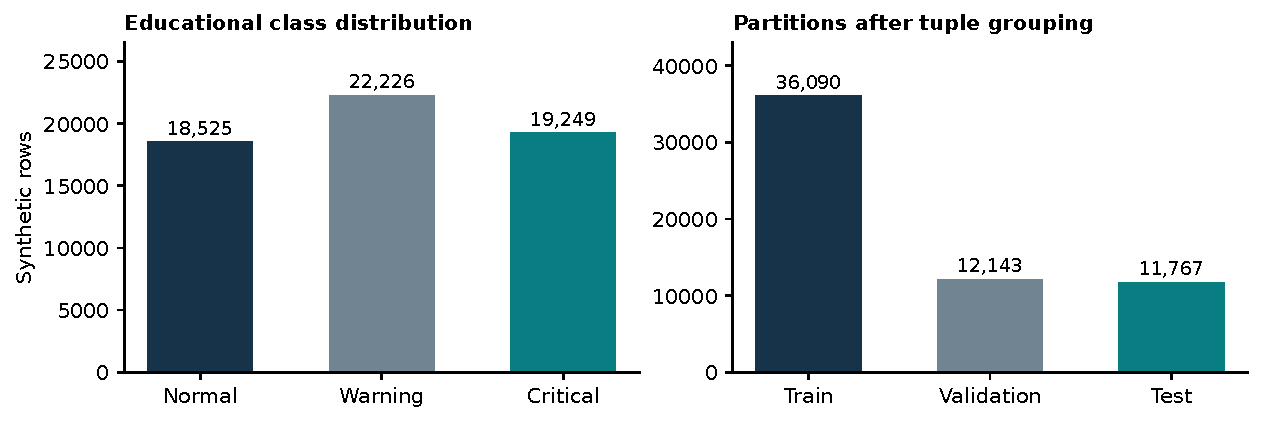
\includegraphics[width=0.95\textwidth]{dataset_summary.pdf}
\caption{Class balance and row partitions from the saved training metadata. Splitting operates on unique feature tuples, so row proportions differ slightly from 60/20/20. These labels are educational categories.}\label{fig:dataset}
\end{figure}}

\newcommand{\MetricsTable}{%
\begin{table}[htbp]\small\centering
\caption{Local validation and test performance. P, R and F1 are macro averages; all values are percentages. Validation selects the model.}\label{tab:metrics}
\begin{tabular}{@{}llrrrrr@{}}\toprule
Model & Partition & Accuracy & P & R & F1 & Critical R\\\midrule
Logistic regression & Validation & 75.15 & 75.18 & 75.53 & 75.34 & 73.85\\
Random Forest & Validation & 100.00 & 100.00 & 100.00 & 100.00 & 100.00\\\addlinespace
Logistic regression & Test & 75.35 & 75.85 & 76.46 & 76.11 & 76.54\\
Random Forest & Test & 100.00 & 100.00 & 100.00 & 100.00 & 100.00\\\bottomrule
\end{tabular}
\end{table}}

\newcommand{\ConfusionFigure}{%
\begin{figure}[htbp]\centering
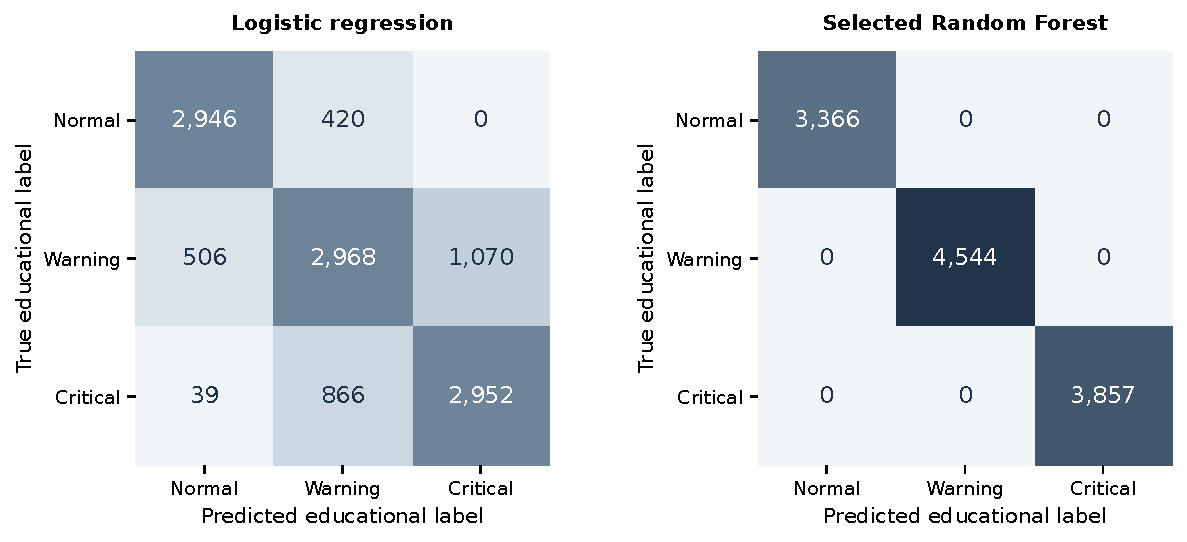
\includegraphics[width=\textwidth]{confusion_comparison.pdf}
\caption{Confusion matrices for 11,767 locally held out synthetic rows. The selected forest reconstructs the rule derived labels perfectly on this split. This is neither clinical validation nor an assessor hidden test.}\label{fig:confusion}
\end{figure}}

\newcommand{\RatesTable}{%
\begin{table}[htbp]\small
\caption{Classification errors and alert observations with explicit denominators. Classifier rates do not measure phone delivery failures.}\label{tab:rates}
\begin{tabularx}{\textwidth}{@{}Y P{32mm}P{31mm}@{}}\toprule
Measure and denominator & Logistic regression & Random Forest\\\midrule
Missed Critical classification: predicted other class / all true Critical & 905/3,857 = 23.46\% & 0/3,857 = 0\%\\
False Warning on Normal: predicted Warning / all true Normal & 420/3,366 = 12.48\% & 0/3,366 = 0\%\\
False Critical on noncritical: predicted Critical / true Normal or Warning & 1,070/7,910 = 13.53\% & 0/7,910 = 0\%\\\midrule
Server episode campaign & \multicolumn{2}{l}{20/20 created; 0/20 duplicate episodes}\\
Missed Critical alert at caregiver phone & \multicolumn{2}{l}{Outside server benchmark scope}\\
False Warning delivered to caregiver & \multicolumn{2}{l}{Outside server benchmark scope}\\\bottomrule
\end{tabularx}
\end{table}}

\newcommand{\VerificationTable}{%
\begin{table}[H]\small
\caption{Current revision and dated baseline verification. Counts are not added because the units and campaigns differ.}\label{tab:verification}
\begin{tabularx}{\textwidth}{@{}P{34mm}P{25mm}Y@{}}\toprule
Evidence & Result & Scope and exclusions\\\midrule
Current Python suite & \CurrentPythonResult & Current revision software record; units are tests\\
Current JVM suite & \CurrentJvmResult & Pure Java checks; not Android runtime acceptance\\
Metric history suite & \CurrentHistoryResult & Weighted means, validity, gaps, boundaries, retention and consent\\
Learning record suite & \CurrentLearningResult & Synthetic persistence, idempotency, authorisation and revocation\\
Current Android scope & Code \CurrentVersionCode & \CurrentAndroidResult\\
Current HTTPS scope & \CurrentIntegrationResult & Distinct from physical Bluetooth or caregiver delivery\\\midrule
Baseline Python/JVM & 88 / 2,830 & 26 October records: Python tests / JVM assertions\\
Baseline HTTPS & 17/17 checks & Loopback TLS, fictional accounts; no phone or Bluetooth\\
Baseline APK and UI & Code 13; 709 checks & Installed on Samsung SM-S948B, Android 17; registration at 200\% font scale. APK SHA-256 \texttt{417c12ef\ldots206378}\\
Baseline benchmark & 20/20 episodes & Temporary databases; no duplicate retry or sustained episodes\\\bottomrule
\end{tabularx}
\end{table}}

\newcommand{\TimingTable}{%
\begin{table}[H]\small
\caption{26 October baseline server processing measurements in milliseconds. Percentiles use linear interpolation; no transport or Android latency is included.}\label{tab:timing}
\begin{tabularx}{\textwidth}{@{}Y rrrr@{}}\toprule
Timed operation & N & Mean & p50 & p95\\\midrule
Warm authenticated classification & 25 & 17.34 & 16.85 & 19.87\\
Third qualifying reading and episode commit & 20 & 7.08 & 6.95 & 9.09\\
Third reading through authenticated inbox GET & 20 & 12.24 & 12.02 & 15.02\\
Cold classification including model load & 1 & 1,059.29 & --- & ---\\\bottomrule
\end{tabularx}
\smallskip\par\footnotesize The first two episode samples were already stored. Inbox timing uses the fictional adult's inbox; caregiver fanout is verified separately by the HTTPS integration fixture.
\end{table}}

\newcommand{\HardwarePhotoFigure}{%
\begin{figure}[htbp]\centering
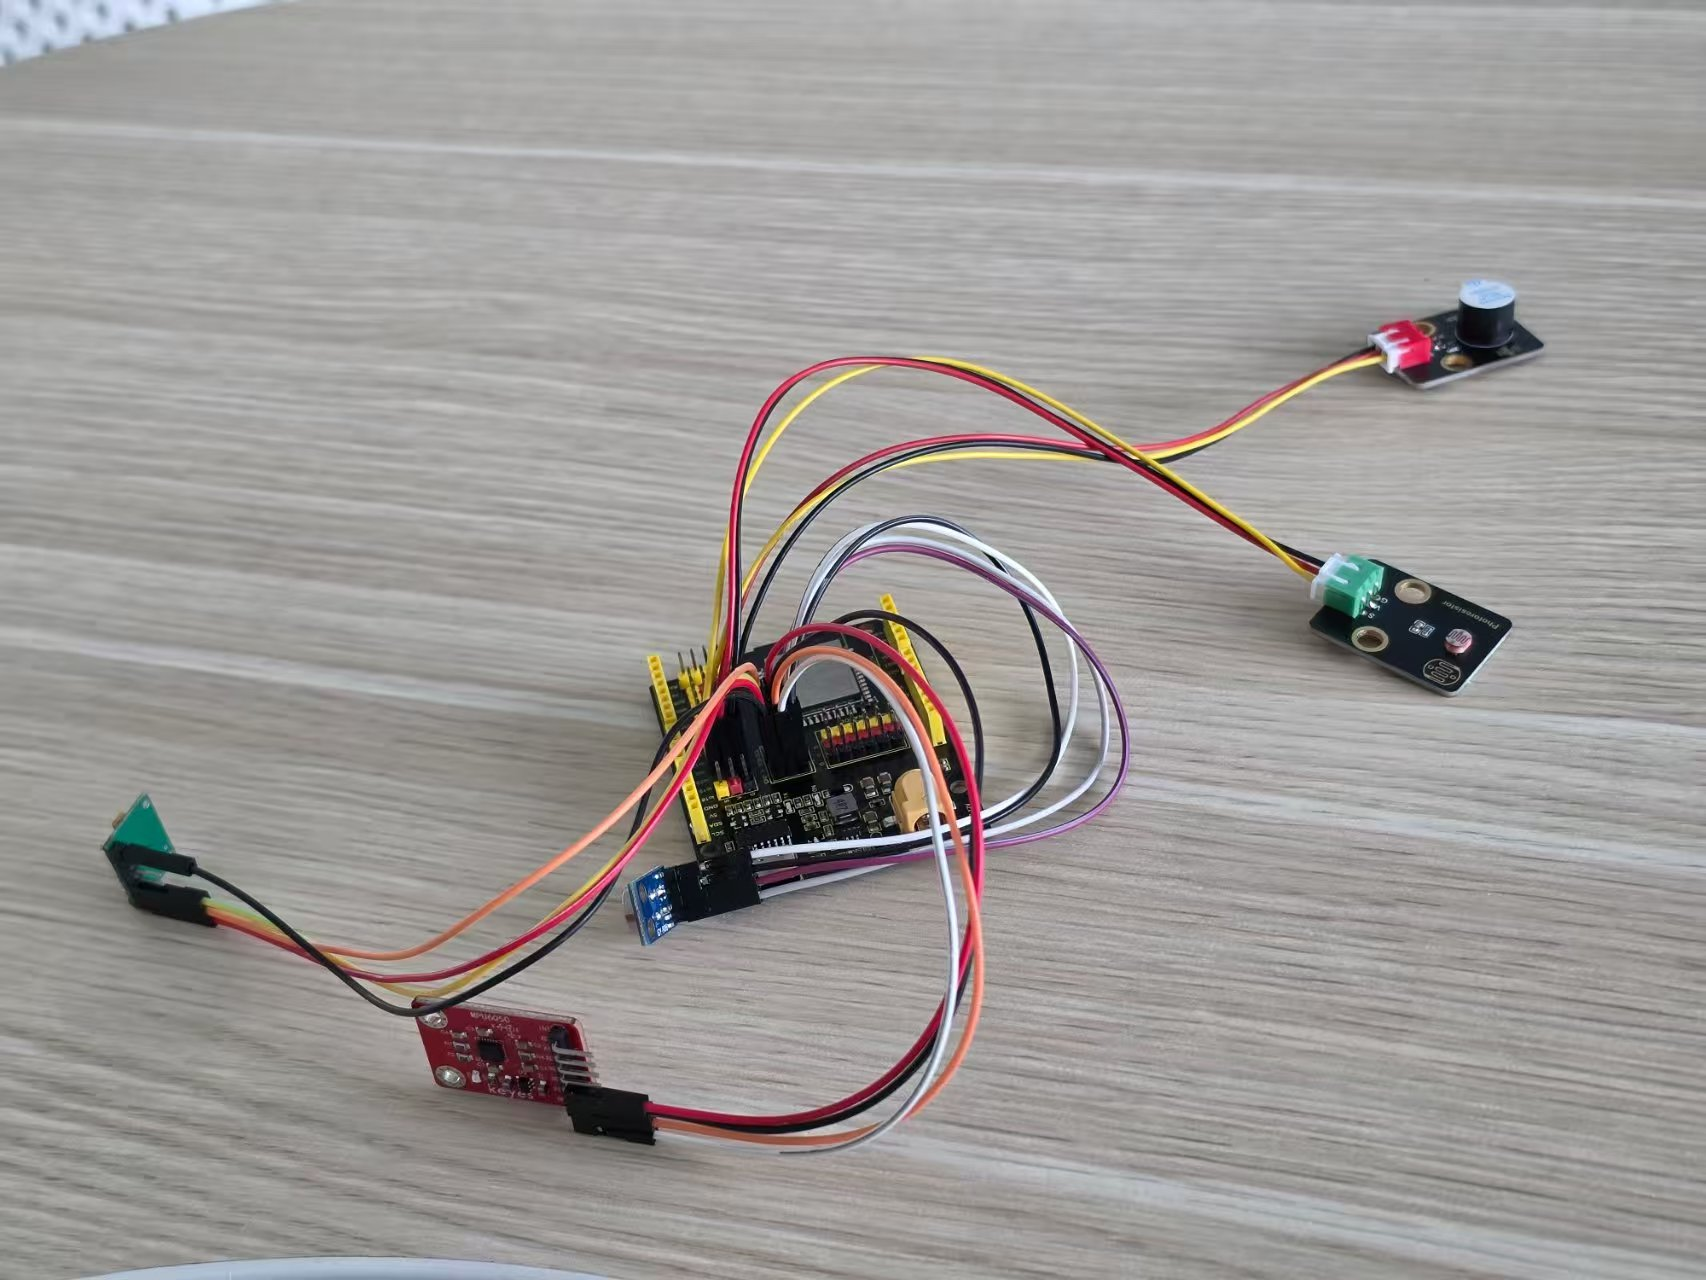
\includegraphics[width=.94\textwidth]{hardware_prototype.jpg}
\caption{Earlier physical prototype photograph supplied by the team. The KEYES carrier and sensor modules document the bench assembly before the microphone and light sensor were removed. The current four-module wiring map is Figure~\ref{fig:wearable-wiring}; this older photograph is not presented as a photograph of the revised arrangement.\cite{hardwarephoto}}\label{fig:hardware-photo}
\end{figure}}
\newcommand{\RoleScreensFigure}{%
\begin{figure}[htbp]\centering
\begin{subfigure}[t]{.45\textwidth}\centering
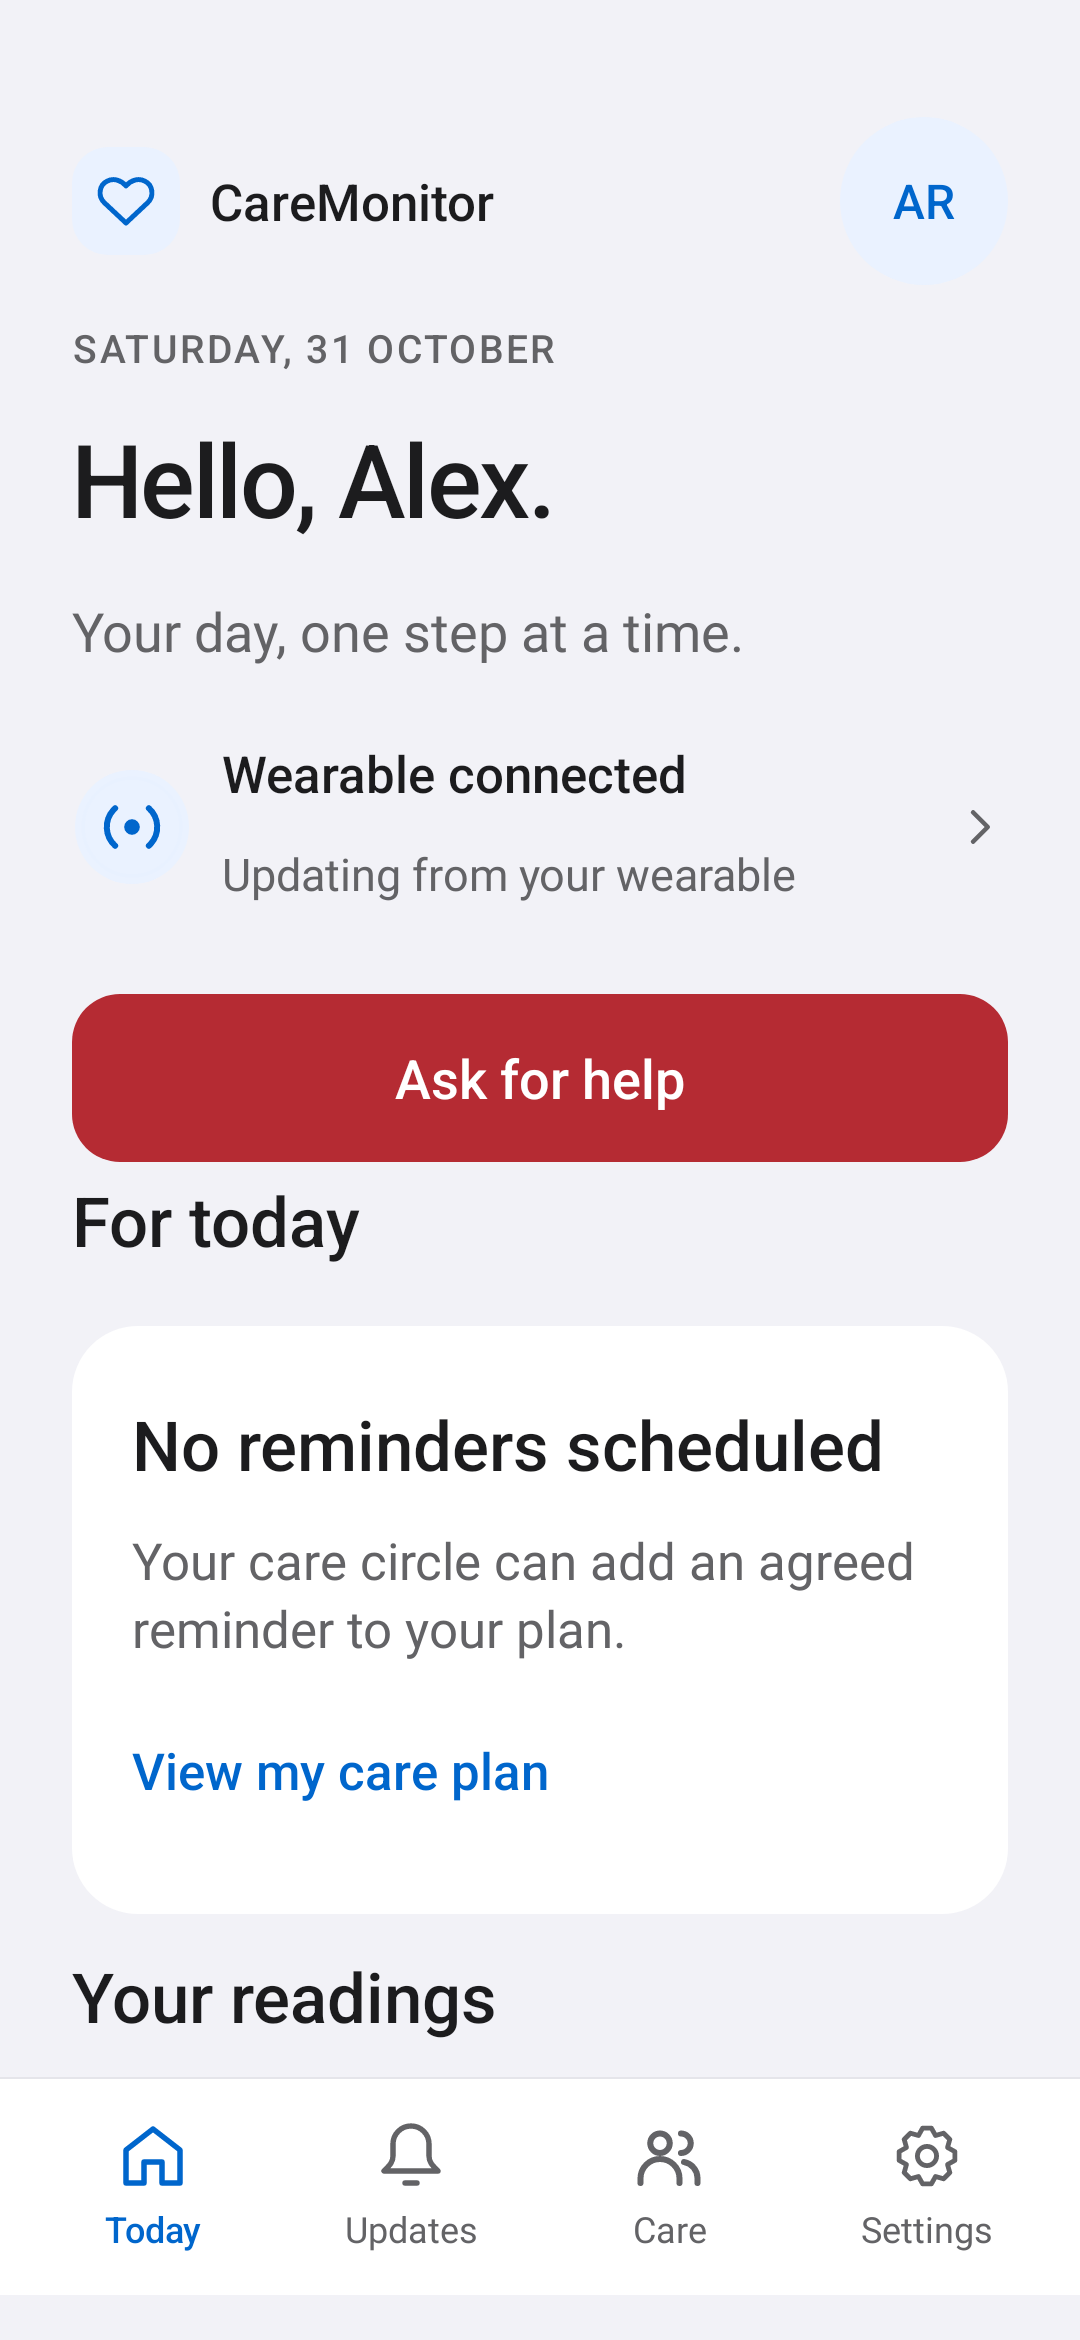
\includegraphics[width=\linewidth,height=.67\textheight,keepaspectratio]{system/elder_live_home_top.png}
\caption{Older adult during authenticated physical reception.}
\end{subfigure}\hfill
\begin{subfigure}[t]{.45\textwidth}\centering
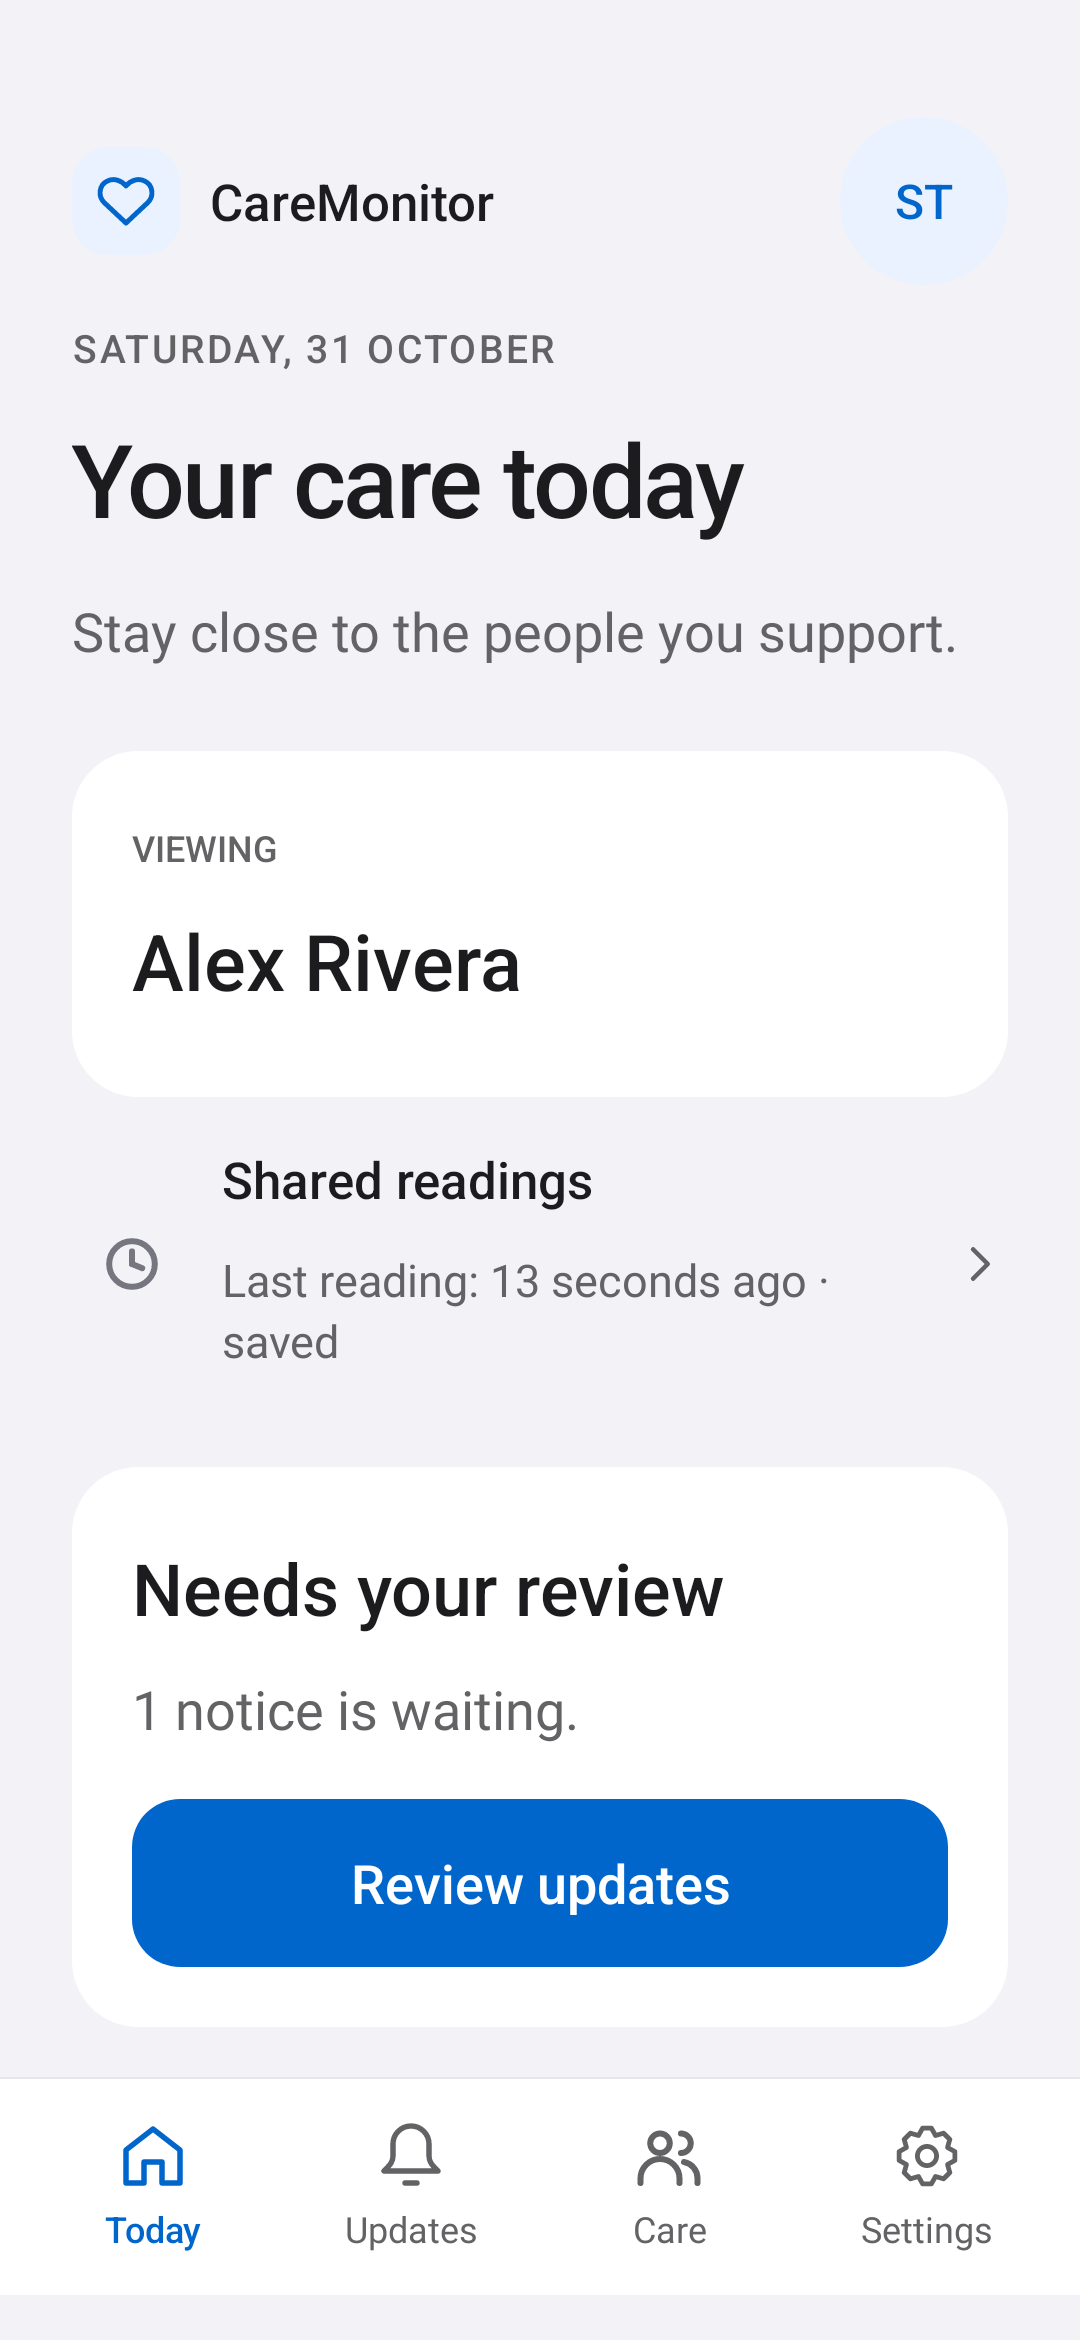
\includegraphics[width=\linewidth,height=.67\textheight,keepaspectratio]{system/caregiver_home_top.png}
\caption{Caregiver: selected person and notices to review.}
\end{subfigure}
\caption{Code 20 production-view captures on S22 / Android 13, using real HTTPS test accounts in an isolated package/database and 100\% text. The adult is captured during physical SPP reception; the caregiver is captured later after an approved link, reminder and controlled help event. These are successive observations, not simultaneous phones or in-memory fixtures. Full provenance and additional views appear in Appendix~\ref{app:usb-run}.}\label{fig:role-screens}
\end{figure}}
\begin{document}
\hypersetup{pageanchor=false}
\begin{titlepage}
\thispagestyle{empty}
{\sffamily\small IOT308TC\quad /\quad ASSESSMENT 2\par}
\vspace{23mm}
{\sffamily\bfseries\fontsize{36}{40}\selectfont IndiCare\par}
\vspace{5mm}
{\sffamily\fontsize{21}{26}\selectfont Mobile IoT monitoring\par}
{\sffamily\fontsize{16}{22}\selectfont Technical report and evaluation\par}
\vspace{12mm}
{\large Wearable sensing, native Android care and\par secure self-hosted analytics\par}
\vspace{16mm}
\begin{tabularx}{\textwidth}{@{}P{39mm}Y@{}}
Team members & \ReportMembers\\
Tutor & \ReportTutor\\
Report date & \ReportDate\\
Repository & \url{https://github.com/deepdevjose/Older-Monitoring-Wearable}\\
\end{tabularx}
\vfill
\colorbox{light}{\parbox{\dimexpr\textwidth-2\fboxsep\relax}{\small\textbf{Educational use only}\par
This prototype must not be used for diagnosis, treatment or clinical decision making. Evaluation separates synthetic model exercises, Android checks and controlled physical bench observations.}}
\end{titlepage}
\pagenumbering{roman}
\hypersetup{pageanchor=true}
\tableofcontents
\clearpage
\pagenumbering{arabic}
\section{Purpose and assessment scope}
\label{sec:purpose}
\begin{reportprose}
IndiCare examines how an Android gateway, a local REST service and introductory machine learning support an educational monitoring workflow. The application is named CareMonitor 1.0.0. Its evaluated capabilities include persistent synthetic alert episodes, consent based access, a reproducible classification service and native Android account navigation. The evidence combines software tests, isolated HTTPS integration, installation on a Samsung phone and targeted interface instrumentation. Each result is attributed to the layer actually exercised.

The assessment covers patient and caregiver views, three class predictions, confidence, storage, alerts and measurable improvement. Mobile functionality and programming architecture carry 45\% of the rubric, making the distinction between server capabilities and visible application behaviour central to the evaluation. This report maps requirements to code, presents quantitative results and analyses the implemented system's coverage. The assessment uses the current versioned API and release records rather than treating historical development captures as proof of current behaviour.\cite{rubric,snapshot}

Classification uses synthetic educational labels. Participant measurements, clinical records and induced falls are outside this study. Historical screenshots document technical development without presenting personal physiological values. A separate SisFall experiment is excluded from the reported classification results. The evaluated CSV is identified as a repository dataset; institutional approval or equivalence to a module supplied dataset is not inferred from its presence. This preserves the distinction between reproducibility, assessment provenance and clinical validity.
\end{reportprose}

\section{Requirements and system architecture}
\label{sec:architecture}
\begin{reportprose}
The primary actors are an adult account, corresponding to the rubric's patient role, and an explicitly authorised caregiver. An adult can approve several caregivers and revoke their access independently. Requirements follow a reading through provenance, validation, transfer, persistence, presentation and alert review. Table~\ref{tab:requirements} associates these behaviours with implementation locations and the evidence available for each one.

Figure~\ref{fig:architecture} distinguishes two implemented server paths. Synthetic snapshots enter the readings service and exercise transparent alert rules, persistent history and private notification inboxes. Synthetic feature vectors enter the classification endpoint and produce a model label and confidence. These services operate independently: the Android care interface retrieves readings and alerts, while its Activity does not consume the classification endpoint. Classification results therefore establish API behaviour, without establishing prediction or confidence presentation on the phone.

A local FastAPI service keeps Python validation, models and account authorisation together. Central inference avoids distributing model updates to every phone but depends on server availability. SQLite offers transactional episode creation with modest deployment complexity. Its single writer architecture suits the evaluated scale; the experiments do not establish large deployment capacity. Native Android Java provides Bluetooth and foreground service access without introducing a cloud service. This describes the technical choice without inferring administrative approval of a particular framework.

The optional ESP32 path supplies device diagnostics over Bluetooth Serial Port Profile to the Android gateway. Source labels distinguish diagnostics from synthetic assessment data. Server inference rejects device sources because synthetic body temperature is not interchangeable with the available surface temperature measurement. HTTPS protects phone to server communication; Bluetooth pairing forms a separate trust boundary. Account and resource authorisation apply independently of either transport.

Observable invariants guide evaluation. A retry preserves one record per sample, and sustained abnormal input preserves one active episode per signal. Unauthorised requests disclose no patient data, while unavailable predictions retain an explicit unknown or error state. Accessibility evidence covers enlarged registration text and control geometry on the installed phone. Timing results are reported as measured baselines because the supplied specification defines no numeric response or delivery threshold. A measured value is consequently distinguished from a formally satisfied timing requirement.
\end{reportprose}
\RequirementsTable
\ArchitectureDiagram
\FloatBarrier

\section{Hardware and data boundaries}
\label{sec:hardware}
\begin{reportprose}
The wearable source integrates an ESP32, MAX30102 optical module, MPU6050 motion module, GY906 temperature module and photoresistor. Sensor status accompanies snapshots so that missing or warming signals need not become plausible numeric measurements. The light channel is an uncalibrated environmental indicator; darkness alone does not establish wear. Surface temperature cannot establish fever, and the installed modules do not measure blood pressure or hydration.

The optical pipeline uses a rolling sample window and validity flags. These are signal handling choices rather than evidence of physiological accuracy. The recorded USB diagnostic contains 25 JSON messages at approximately one message per second, with optical no contact, the motion module offline and the temperature module online. It retains no physiological values. Firmware compilation and this diagnostic observation are separate evidence: neither identifies the installed binary by a verified hash.\cite{snapshot}

Figure~\ref{fig:hardware-photo} presents the supplied photograph of the physical ESP32 assembly, modules and wiring. It documents the assembled hardware and complements the functional architecture diagram. Visible components and connections alone do not demonstrate sensor calibration, firmware identity or successful data delivery. The historical serial and HTTP captures in Appendix~\ref{app:images} similarly establish development activity under their displayed versions. Hardware is an extension of the synthetic monitoring study, whose classification results are evaluated separately from physical measurements.
\end{reportprose}
\HardwarePhotoFigure
\FloatBarrier

\section{Mobile behaviour and programming structure}
\label{sec:mobile}
\begin{reportprose}
The Android application implements registration, login, adult and caregiver navigation, reading summaries, alert history and settings. Registration introduces the role before collecting name, email and password in four progressive steps. Server configuration belongs to authenticated Settings, keeping technical connection details outside the initial account form. Wearable setup is restricted to the adult role; caregivers use the relationship request and approval workflow. Separate accounts and server enforced revocation prevent shared credentials or locally hidden controls from becoming the access model.

Progressive registration presents one category of information at a time and preserves the draft when the user moves backwards. The primary action stays available while the inputs scroll, making the current step and its completion control identifiable at enlarged text. Password visibility is an explicit user choice, with masking enabled initially. These are concrete interaction decisions supported by instrumentation, rather than a claim of measured preference or reduced cognitive burden. Role selection also determines the subsequent task: the adult configures a wearable, while the caregiver seeks authorised access to another account.

The interface combines labelled cards, text status, icons and large controls. A Samsung SM-S948B running Android 17 hosted version 1.0.0, code 13. Its instrumentation passed 709 checks, including role selection, preserved registration drafts, password masking, navigation and authenticated connection settings. Registration forms were exercised with per Activity font scale 2.0, scrollable inputs and a visible fixed primary action with targets of at least 56 dp. These observations support that specific layout claim; they do not establish a manual TalkBack evaluation or every screen at enlarged text.\cite{accessibility,validation}

Figure~\ref{fig:mobile-layers} shows a layered, MVC inspired arrangement. MainActivity constructs views and coordinates state, combining presentation control with view composition. ReadingSummary, LiveSampleFreshness and AlertInbox encapsulate behaviour testable outside Android. ApiClient and ApiSession manage requests and account state, SecureStore protects persistence, and SensorTransport separates Bluetooth implementations. This is partial separation of concerns rather than a complete MVVM architecture. Android's guidance provides a useful basis for assessing the boundary between interface orchestration and reusable data responsibilities.\cite{androidarch}

Bluetooth acquisition and queued relay use dedicated services and workers. Network tasks run through an executor, with interface changes posted to the main thread. Session and lifecycle checks prevent callbacks from an earlier screen or account from becoming current state. Notification service activation uses an explicit user action and visible foreground notification. The interface instrumentation preserved permissions, preferences, session and outbox state and created no server accounts, separating controlled UI checks from a real authentication or Bluetooth campaign.

The reading history endpoint and SensorChartView exist, but the Activity neither requests that history nor mounts the chart. The classification API likewise returns three classes and confidence without a corresponding mobile prediction widget. These are precise coverage boundaries for the rubric's mobile history and inference criteria. The installed application's verified navigation and registration behaviour are assessed alongside those boundaries, without promoting compilation or instrumentation into complete sensor to caregiver operation.
\end{reportprose}
\MobileLayersDiagram
\RoleTable

\section{REST integration storage and alert lifecycle}
\label{sec:integration}
\begin{reportprose}
The API uses the prefix \code{/api/v1}. Users authenticate through account endpoints and send a Bearer session token. Readings carry a stable sample identifier, capture timestamp, source and structured payload. Pydantic contracts reject malformed or unsupported inputs, while account and resource checks enforce access. Appendix~\ref{app:api} records endpoint details and an observed synthetic prediction, making the current contract explicit.\cite{api}

The phone queue retains snapshots during temporary upload failure. Reusing a sample identifier makes a retry idempotent: a lost response creates neither another sample nor another alert. The server writes reading state, alert state and private notification entries transactionally. SQLite isolation lets readers observe committed changes; it does not guarantee delivery to a disconnected handset.\cite{sqlite} Figure~\ref{fig:sequence} traces a qualifying upload through storage and fanout to two approved caregivers.

The outbox stores each item before transmission and removes it after acknowledgement. Its capacity is two hundred items, so the design does not imply lossless indefinite disconnection. Items retain account and endpoint ownership to prevent relay across sessions. Authentication, permission and validation errors pause sending; transient failures use retry and backoff. Policy tests exercise these decisions. Actual process termination, AndroidKeyStore persistence and subsequent physical delivery form a different device execution boundary from those tests.

Synthetic rule episodes require three recent valid samples with distinct timestamps separated by one to thirty seconds. Sustained abnormal input creates one unresolved episode per signal. Further abnormal samples update its evidence without repeatedly creating the same episode. Three eligible observations no longer triggering the rule recover it. Missing contact, disconnected sensors and invalid values cannot close an episode because unusable evidence does not establish recovery. Figure~\ref{fig:alert-state} makes these transitions explicit.

Acknowledgement records caregiver specific review rather than recovery. One caregiver's action does not suppress another caregiver's history. Delivery acknowledgement is also distinct from review. A persistent private inbox and authenticated long polling support recovery after interruption, while the reported timing experiments measure server processing rather than Android notification arrival.

The synchronous classification route runs through FastAPI's thread pool.\cite{fastapi} Two bounded inference slots and a per account request limit constrain work. A successfully loaded model is cached; an unavailable or busy model produces an explicit error instead of a fabricated normal prediction. JSON inference responds without creating a stored reading or alert. Model confidence therefore does not drive the rule episodes evaluated in this report.
\end{reportprose}
\SequenceDiagram
\AlertStateDiagram

\section{Synthetic classification and model evaluation}
\label{sec:ml}
\begin{reportprose}
The experiment reads the 60,000 row repository CSV using pandas. It retains three numeric features: synthetic heart rate, oxygen saturation and body temperature. Identifiers, other measurements and alert columns are excluded from the feature matrix. Missing, nonnumeric or nonfinite values fail preparation instead of being interpreted as healthy. Targets count abnormal flags across the three alert columns: zero gives Normal, one Warning, and two or three Critical. These constructed educational categories have no independent clinical ground truth.\cite{mlartifact}

Repeated feature tuples could place identical examples in training and evaluation. The training script groups the 18,939 unique feature tuples before a stratified split with seed 42. Every occurrence of one tuple stays in one partition. The resulting counts are 36,090 training, 12,143 validation and 11,767 test rows. This controls exact tuple leakage without creating external validation. The test partition is a local holdout, not an assessor controlled hidden test set.

Two introductory supervised classifiers are compared. Logistic regression uses StandardScaler fitted within its training pipeline, balanced class weights and at most 2,000 iterations. Random Forest uses 120 trees, maximum depth fourteen, minimum leaf size two and balanced class weights. Validation macro F1 selects the model, with Critical recall as tie breaker. Test results are reported after selection rather than used to select. Random Forest reaches validation macro F1 of 1.0000 against logistic regression's 0.7534 and is saved for endpoint inference.

Table~\ref{tab:metrics} reports accuracy and macro precision, recall and F1. Macro averaging weights categories equally; Critical recall also exposes missed critical classifications.\cite{sklearn} Figure~\ref{fig:confusion} presents both confusion matrices with true classes as rows. Logistic regression misclassifies 905 of 3,857 Critical examples and assigns Warning to 420 of 3,366 Normal examples. Random Forest makes no observed holdout errors. Table~\ref{tab:rates} defines the corresponding rates and denominators.

The perfect forest result reflects reconstruction of deterministic synthetic boundaries rather than medical reliability. Robustness to another generator, sensor noise or distribution shift is outside this experiment. Confidence is the largest predict\_proba score, rounded to six decimals. It is not calibrated against real outcomes and cannot represent the probability of disease or emergency. The inference contract requires fresh synthetic features within recorded training ranges. Before deserialisation, the local model file is hash checked and its scikit learn version compared with metadata. This mechanism does not make untrusted model files safe to load.

Logistic regression offers an interpretable baseline, but linear decision surfaces cannot readily represent every disconnected region created by combinations of threshold flags. A tree ensemble represents those combinations more directly. This interpretation is consistent with the matrices without establishing a unique explanation for each error. Reporting all classes prevents a favourable average from concealing weak Critical recall. The result is a reproducible local model comparison whose synthetic targets and dataset provenance delimit its interpretation.

Evaluation keeps feature preparation, model selection and final reporting distinct. Scaling is learned from training data rather than the complete dataset, and validation guides selection before the holdout is inspected for the reported comparison. Grouping prevents duplicate feature tuples from inflating performance through exact repetition across partitions. It does not remove the shared rule generator behind all three partitions. The resulting high score is therefore informative about reconstruction of the supplied synthetic task, while generalisation to a new population is a separate scientific question.
\end{reportprose}
\DatasetFigure
\MetricsTable
\ConfusionFigure
\RatesTable

\section{Security configuration and development evidence}
\label{sec:security}
\begin{reportprose}
Accounts use Argon2id password hashes and random session tokens with hashed server representations. Resource access requires the correct role and an active approved relationship to the adult. Invitation codes request access without independently authenticating caregivers or disclosing readings. Expiry, limited attempts and adult approval constrain guessing. Argon2id follows established storage guidance; its inclusion is an implementation property rather than evidence of a comprehensive security audit.\cite{owasp}

HTTPS verifies certificate names. Sensitive server fields use authenticated AES GCM encryption, while Android protects stored state through its KeyStore backed store. Identifiers, timestamps and event types are visible database metadata. Private configuration, database state and signing material are excluded from version control. The checked in server certificate is public trust material, and backups use a passphrase with restoration invalidating sessions. These distinctions define the protection actually provided.

Repository history records development under one contributor identity. It establishes versioned changes without identifying each student's personal responsibility, controlled peer review or agreed contribution factor. Appendix~\ref{app:contribution} presents the supplied four member roster and student IDs alongside the attribution basis. The report makes no individual authorship claim from a shared repository identity and does not infer equal effort from membership alone. This treats collaboration evidence as an attribution question separate from software correctness.\cite{git}
\end{reportprose}

\section{Testing measured outcomes and improvement}
\label{sec:testing}
\begin{reportprose}
Current release records report 88 passing Python tests, 2,830 JVM assertions and seventeen passing HTTPS integration checks. Device instrumentation adds 709 targeted Android interface checks. These are different measurement units, reported separately in Table~\ref{tab:verification}. The HTTPS fixture uses fictional accounts, strict hostname verification and two authorised caregivers. It covers revocation, independent review, idempotent retry and model serving. The device campaign tests onboarding and navigation rather than extending that fixture through Bluetooth and the phone network.\cite{validation,integration}

A reproducible benchmark uses disposable databases and an in process ASGI TestClient. Twenty five warm classification requests produce mean response time 17.34 milliseconds and p95 19.87 milliseconds. The first request takes 1,059.29 milliseconds, including lazy model loading. Twenty independent synthetic pulse episodes produce p95 9.09 milliseconds for third qualifying ingestion and 15.02 milliseconds from immediately before ingestion until an authenticated inbox read completes. All twenty retry and sustained sample checks retain one unresolved episode.\cite{benchmark}

These measurements exclude TLS, network transport, the preceding sampling interval, long polling and Android rendering. They establish local server processing rather than caregiver alert latency. Table~\ref{tab:timing} records boundaries and sample counts. Likewise, classifier false warnings and missed Critical labels describe holdout prediction errors, not complete application delivery failures. Keeping these denominators distinct makes both performance and reliability claims interpretable.

The forest improves test accuracy by 24.65 percentage points and macro F1 by 23.89 points over logistic regression. A separate chronological backend experiment compares the initial server at commit 6757c0a with the evaluated implementation. Both receive twenty distinct synthetic samples twice, representing a lost response and retry. The initial server stores forty rows; the evaluated server stores twenty, with every retry reusing its existing identifier. This removes twenty duplicate rows in the matched campaign. The adapter script documents the different contracts. The result demonstrates improved persistence semantics rather than faster operation or mobile inference integration.\cite{improvement}

Scenario coverage distinguishes deterioration from malformed input. Valid synthetic sequences progress from normal values to sustained abnormal conditions and recovery. Missing fields, nonfinite values, stale timestamps and absent optical contact instead cause rejection or preserve unknown state. Retry policies and lost responses exercise network failure decisions; unlinked and revoked caregivers exercise authorisation. Appendix~\ref{app:repro} specifies the measurement protocol and separates executable software scenarios from physical transport and operating system behaviour.

The combined evidence supports precise conclusions: server alerts persist without retry duplication, model results are reproducible, and progressive account setup renders on the installed Android release. Physical Bluetooth pairing, complete phone to server delivery, manual screen reader use and mobile prediction display are outside the demonstrated coverage. Those boundaries constrain the rubric interpretation without weakening the observed results or suggesting that one test layer substitutes for another.
\end{reportprose}
\VerificationTable
\TimingTable

\section{Conclusion}
\begin{reportprose}
IndiCare demonstrates a local architecture with persistent synthetic alerts, explicit access control, a reproducible two model comparison and verified Android onboarding. Random Forest reproduces the synthetic holdout labels, while idempotent ingestion halves stored rows in the matched retry campaign. The installed application's progressive role based registration is supported by targeted device evidence. Classification confidence is an API capability, and physical transport and clinical effectiveness are outside the demonstrated results. The report's contribution is a traceable educational evaluation that connects each quantitative claim to its actual data, implementation layer and measurement boundary.
\end{reportprose}

\FloatBarrier
\clearpage
\begin{thebibliography}{99}
\addcontentsline{toc}{section}{References}
\small
\bibitem{rubric} IOT308TC. \emph{Assessment 2 AI Enabled Mobile IoT Healthcare Monitoring Application}. Supplied assessment brief and marking rubric, \path{rubrik.docx}. 3,000 words $\pm$10\%; eight weighted criteria.
\bibitem{snapshot} IndiCare project. \emph{CareMonitor 1.0.0 implementation and acceptance status}. Repository commit \texttt{5c650c1}, \path{README.md}, \path{docs/STATUS.md}, \path{docs/SECURITY_ETHICS.md} and \path{release/FIRMWARE_DIAGNOSTIC.json}. \url{https://github.com/deepdevjose/Older-Monitoring-Wearable}.
\bibitem{api} IndiCare project. \emph{Versioned API and implementation}. \path{docs/API.md}, \path{server/caremonitor/api.py}, \path{schemas.py}, \path{alerts.py}, \path{db.py}, \path{routes_ml.py} and Android source in \path{mobile/app/src/main/java/org/caremonitor/demo/}.
\bibitem{mlartifact} IndiCare project. \emph{Synthetic health model training and evaluation}. \path{tools/train_models.py}; \path{models/synthetic-health-v1/metadata.json}. Seed 42; scikit learn 1.8.0. Snapshot included as \path{evidence/model-metadata.json}.
\bibitem{validation} IndiCare project. \emph{Release software validation, Android build and device interface checks}. \path{evidence/VALIDATION.json}, \path{ANDROID_BUILD.json}, \path{ANDROID_UI_EVIDENCE.json}, \path{pytest-current.xml} and \path{jvm-current.txt}, 26 October 2026. APK code 13; 709 checks on Samsung SM-S948B with Android 17.
\bibitem{hardwarephoto} IndiCare team. \emph{Physical prototype assembly photograph}. Supplied 26 October 2026; reproduced as \path{figures/hardware_prototype.jpg}. Original source path and SHA-256 recorded in \path{evidence/hardware_photo.json}.
\bibitem{integration} IndiCare project. \emph{Isolated HTTPS integration evidence}. \path{release/INTEGRATION_EVIDENCE.json}, 25 October 2026. Seventeen checks; fictional accounts; no physical phone.
\bibitem{benchmark} IndiCare report audit. \emph{Current server processing benchmark}. \path{tools/benchmark_api.py} and \path{evidence/benchmark-current.json}, 26 October 2026. In process ASGI, temporary databases; raw samples and boundaries retained.
\bibitem{improvement} IndiCare report audit. \emph{Lost response retry comparison}. \path{tools/benchmark_idempotency.py} and \path{evidence/idempotency-before-after.json}, 26 October 2026. Initial \texttt{6757c0a:main.py} compared with current API using twenty matched synthetic pairs.
\bibitem{git} IndiCare project. \emph{Main branch version history}. Four commits, 25--26 October 2026; evidence in Appendix~\ref{app:contribution}. \url{https://github.com/deepdevjose/Older-Monitoring-Wearable/commits/}.
\bibitem{fastapi} FastAPI. \emph{Concurrency and async await}. Official documentation. \url{https://fastapi.tiangolo.com/async/}. Accessed 26 October 2026.
\bibitem{sklearn} Scikit learn. \emph{Metrics and scoring quantifying the quality of predictions}. Version 1.8 documentation. \url{https://scikit-learn.org/1.8/modules/model_evaluation.html}. Accessed 26 October 2026.
\bibitem{androidarch} Android Developers. \emph{Guide to app architecture}. Official documentation. \url{https://developer.android.com/topic/architecture}. Accessed 26 October 2026.
\bibitem{accessibility} Android Developers. \emph{Make apps more accessible Views}. Official documentation. \url{https://developer.android.com/guide/topics/ui/accessibility/views/apps-views}. Accessed 26 October 2026.
\bibitem{owasp} OWASP. \emph{Password Storage Cheat Sheet}. \url{https://cheatsheetseries.owasp.org/cheatsheets/Password_Storage_Cheat_Sheet.html}. Accessed 26 October 2026.
\bibitem{sqlite} SQLite. \emph{Isolation in SQLite}. Official documentation. \url{https://www.sqlite.org/isolation.html}. Accessed 26 October 2026.
\end{thebibliography}

\clearpage
\appendix
\section{API contract and synthetic example}
\label{app:api}
All paths below use \code{/api/v1}. A session is required except for registration and login. Exact validation and error bodies are defined by the source, not the historical screenshots.

\begin{longtable}{@{}P{19mm}P{69mm}P{65mm}@{}}
\caption{Selected current REST operations.}\label{tab:api}\\
\toprule Method & Path & Purpose and access\\\midrule\endfirsthead
\toprule Method & Path & Purpose and access\\\midrule\endhead
POST & \path{/auth/register}, \path{/auth/login} & Create an educational account or start a session\\
GET/POST & \path{/me}, \path{/auth/logout} & Read own profile or revoke current session\\
POST & \path{/readings} & Adult uploads own source labelled snapshot; idempotent sample ID\\
GET & \texttt{/patients/\{id\}/overview} & Current reading and care state; own or approved resource\\
GET & \texttt{/patients/\{id\}/readings} & Persisted reading history; own or approved resource\\
GET & \texttt{/patients/\{id\}/alerts} & Stored alert episodes; own or approved resource\\
POST & \texttt{/alerts/\{id\}/acknowledge} & Record the approved caregiver's own review\\
GET & \path{/notifications}, \path{/notifications/wait} & Private durable inbox or authenticated long poll\\
GET & \path{/ai/model} & Educational model identity and limitations\\
POST & \path{/ai/classify} & Synthetic features to class and confidence; no automatic reading or episode persistence\\\bottomrule
\end{longtable}

\subsection{Observed inference request and selected response fields}
The following normal example is retained in \path{evidence/benchmark-current.json}. Values are synthetic fixtures. Confidence is a model class score. The complete response also includes the model limitations.
\begin{lstlisting}
POST /api/v1/ai/classify
Authorization: Bearer <session supplied at runtime>

{
  "source": "synthetic",
  "features": {
    "heart_rate_bpm": 75.0,
    "spo2_percent": 98.0,
    "body_temp_c": 36.5,
    "sample_age_seconds": 0.0
  }
}

{
  "classification": "Normal",
  "confidence": 0.999263,
  "model_id": "synthetic-health-v1",
  "source": "synthetic",
  "educational_only": true
}
\end{lstlisting}

\begin{table}[htbp]\small
\caption{Expected failure behaviour of classification and data endpoints.}
\begin{tabularx}{\textwidth}{@{}P{34mm}Y@{}}\toprule
Condition & Behaviour to demonstrate\\\midrule
Missing or invalid session & Reject protected request; no patient data returned\\
Wrong patient relationship & Deny resource without revealing its contents\\
Missing feature, NaN, stale feature vector or device source & Classification rejected; no invented prediction\\
Same sample ID with changed content & Conflict response; existing sample preserved\\
Prediction limit exceeded & HTTP 429; user can retry later\\
Model unavailable or inference slots occupied & HTTP 503; no invented prediction is returned\\\bottomrule
\end{tabularx}
\end{table}
\FloatBarrier

\section{Reproduction installation and scenario evidence}
\label{app:repro}
\subsection{Evidence package and word count}
The prose count is generated by \path{tools/count_words.py}: \MainWordCount{} words in explicit \code{reportprose} environments. Headings and citation markers are excluded; including the short headings would remain within the permitted range. Tables, figures, title, references, test evidence and appendices are excluded as the assessment specifies. No source code listing appears in the main report.

\begin{tabularx}{\textwidth}{@{}P{50mm}Y@{}}\toprule
Report evidence & Purpose\\\midrule
\path{model-metadata.json} & Training recipe, split, class metrics, artifact hashes and limitations\\
\path{benchmark-current.json} & All current timing samples and measurement boundaries\\
\path{idempotency-before-after.json} & Matched retry campaign with revision IDs and record counts\\
\path{pytest-current.xml} & Current 88 test rerun in JUnit format\\
\path{jvm-current.txt} & Current 2,830 assertion Java run\\
\path{ANDROID_UI_EVIDENCE.json} & 709 interface checks on Samsung SM-S948B; registration at text scale 2.0\\
\path{hardware_photo.json} & Original hardware photograph, source path, copy identity and scope\\
Release JSON snapshots & Code 13 build, software validation, HTTPS integration and diagnostic records\\
\path{crop_manifest.json} & Source image hashes and exact crop coordinates\\\bottomrule
\end{tabularx}

\subsection{Build and isolated checks}
Run the following from the repository root, with its Python environment installed. The benchmark scripts use temporary databases and fictional accounts, not the running server. They write separate rerun files rather than replacing the recorded results. The historic comparison requires Git commit \texttt{6757c0a}; it adapts the legacy unversioned API and current versioned API to the same duplicate delivery campaign. It is not a throughput comparison.
\begin{lstlisting}[language=bash]
python3 docs/report/tools/count_words.py
bash docs/report/build.sh
.venv/bin/python -m pytest tests
.venv/bin/python mobile/scripts/test_reading_summary.py --jdk /usr
.venv/bin/python docs/report/tools/benchmark_api.py
.venv/bin/python docs/report/tools/benchmark_idempotency.py
\end{lstlisting}

\begin{figure}[htbp]\centering
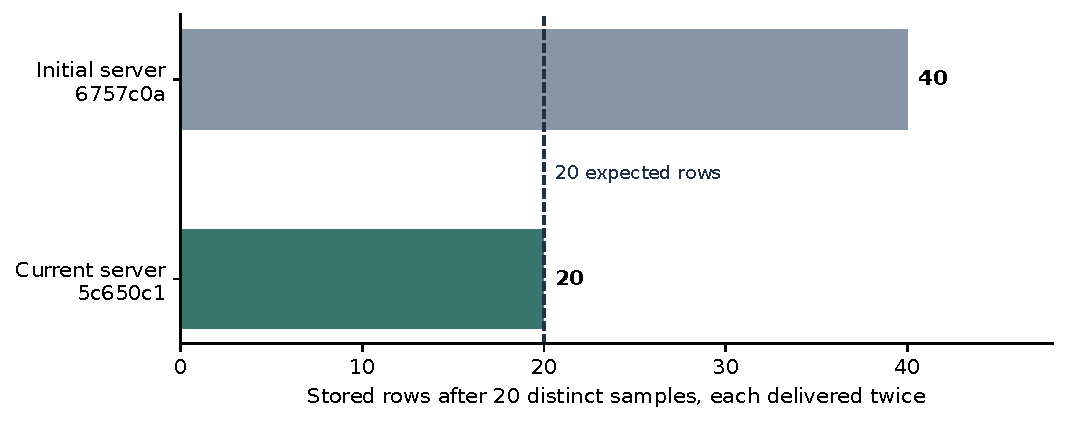
\includegraphics[width=.88\textwidth]{idempotency_improvement.pdf}
\caption{Measured chronological improvement in backend persistence. Forty successful responses represent twenty unique samples delivered twice. The baseline creates twenty extra rows; the current API preserves twenty unique records. The comparison excludes handset and network behaviour.}\label{fig:improvement}
\end{figure}

\subsection{Installation and execution procedure}
The release APK and source archive are distributed under \path{release/}. The recorded APK is version 1.0.0, code 13, minimum API 24 and target API 37. Its SHA-256 is \path{417c12efa634e960b5e3f0ab680a14951b4357a8580f59eb7b7c75caea206378}. Installation and launch on Samsung SM-S948B with Android 17 are recorded alongside 709 native interface checks. The following procedure documents replication of the separate account, server and interface paths. The operational guide is \path{docs/SERVER.md}.
\begin{enumerate}
\item Prepare the Python environment from \path{requirements.txt}; initialise the local server using \code{./carectl init --host YOUR_LAN_IP}. Keep generated keys private.
\item Use \code{./carectl start} and \code{./carectl status} to check HTTPS service readiness. Ensure the public CA bundled in the APK matches that server. Follow \path{docs/SERVER.md} when regenerating a build.
\item Install \path{release/CareMonitor-1.0.0.apk} using Android's authorised local installation flow and retain its hash and device identity. The recorded device uses Android 17/API 37; its interface tests do not grant permissions or activate sensors.
\item Use fictional adult and caregiver accounts for server experiments. Registration presents role, name, email and password as separate steps; the adult issues an invitation and approves the caregiver request. The server enforces that relationship.
\item Run \code{./carectl demo} with fictional adult credentials. This sends three synthetic rule samples; verify one episode and independent caregiver review. This command does not demonstrate a mobile model confidence view.
\item Exercise classification with fixed synthetic features through \path{/api/v1/ai/classify}; inspect the returned class, score and source. Reading persistence and retrieval use the separate readings endpoints. Care navigation and model inference have distinct presentation boundaries.
\item Reproduce the interface campaign with \path{mobile/scripts/test_onboarding_device.py}, selecting the exact device serial. The auxiliary instrumentation checks role selection, back navigation, password masking, enlarged registration forms and authenticated Settings using fictional in-memory profiles.
\end{enumerate}

\clearpage
\subsection{Scenario coverage matrix}
\small
\begin{longtable}{@{}P{24mm}P{62mm}P{67mm}@{}}
\caption{Reproducible scenarios, observed evidence and execution boundaries.}\\
\toprule Scenario & Input and expected result & Recorded evidence and scope\\\midrule\endfirsthead
\toprule Scenario & Input and expected result & Recorded evidence and scope\\\midrule\endhead
Normal & Fixed synthetic normal features; return Normal and score; valid normal snapshots create no rule episode & Model/API execution; classification is a server result, separate from care navigation\\
Deteriorating & Move from eligible normal snapshots to three distinct abnormal snapshots; one episode after persistence & Sustained condition and recovery test in isolated server fixtures\\
Critical & Select known Critical CSV fixture; return expected class; independently exercise an abnormal rule sequence & Held out model matrices and server episode campaign; delivery rate is a separate measure\\
Missing data & Omit required model feature; reject. Missing optical contact must not trigger or recover a rule & Missing feature and invalid contact tests; care views retain explicit unknown states\\
Invalid data & NaN, unexpected field, unsupported feature or stale age; reject classification & \path{test_ml.py}, \path{test_ai_api.py}, request limits tests\\
Network failure & Lose upload response and retry same ID; retain one row and active episode & Matched backend comparison and relay policies; excludes physical radio interruption\\
Unauthorised & Query unlinked adult, then revoke previously approved caregiver; disclose no resource & Server IDOR and revocation tests; native caregiver wearable controls are also rejected\\
Recovery & Three eligible observations no longer meeting the rule; recover episode; later new sustained event may create another & Sustained condition recovery test; review is not recovery\\\bottomrule
\end{longtable}
\normalsize

Exact automated anchors in \path{tests/test_api.py} include \path{test_sustained_condition_one_episode_valid_recovery_then_new_episode}, \path{test_idempotency_conflict_and_capture_order}, \path{test_idor_cannot_read_or_write_other_patients} and \path{test_revoke_removes_data_and_queued_notifications}. Model input boundaries are exercised by \path{tests/test_ai_api.py::test_synthetic_api_rejects_device_and_missing_features}. These names locate executable checks; they do not represent installed Android tests.

\subsection{Application latency and improvement protocol}
Select an initial revision and an improved revision before the experiment. Use the same device, dataset fixture IDs, server hardware, network and permissions. After identical warmup, record at least thirty trials per scenario. Measure API time from dispatch to parsed response, and caregiver latency from the first qualifying synthetic input to visible notification. Keep raw timestamps, request IDs, failed trials and timeouts. Report N, mean, p50 and p95 for both revisions; do not silently omit failed deliveries.

For missed Critical alerts, divide Critical scenarios without a required visible alert within the declared observation window by all Critical scenarios that should generate one. For false Warnings, divide Normal scenarios producing an unwanted Warning by all Normal scenarios. Define the observation window before testing. Model predictions and rule alerts have different semantics; a latency experiment must identify the rule output and its observation window. Separately report duplicates and data loss after reconnection.
\FloatBarrier
\clearpage
\section{Historical development images}
\label{app:images}
The following supplied captures are cropped for relevance. No output or values have been synthesised. Source paths and crop coordinates are recorded in \path{evidence/crop_manifest.json}. They document historical software experiments, separately from the assembly in Figure~\ref{fig:hardware-photo} and the Android code 13 interface campaign.

\begin{figure}[htbp]\centering
\begin{subfigure}{.485\textwidth}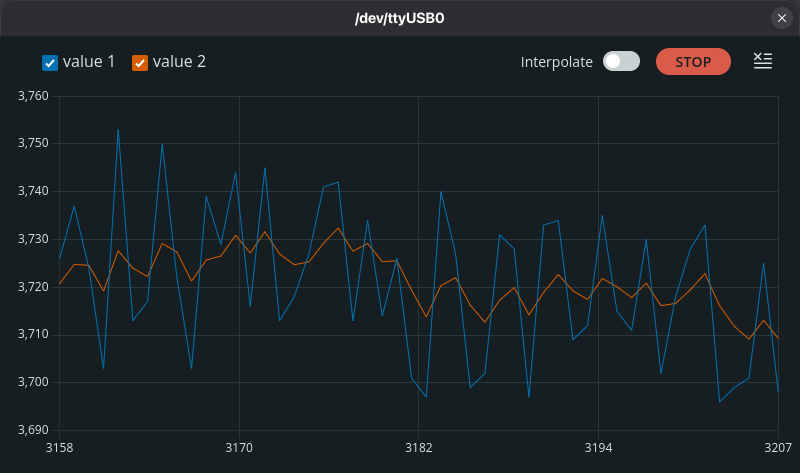
\includegraphics[width=\linewidth]{adc_smoothing.png}\caption{Raw and smoothed ADC traces.}\end{subfigure}\hfill
\begin{subfigure}{.485\textwidth}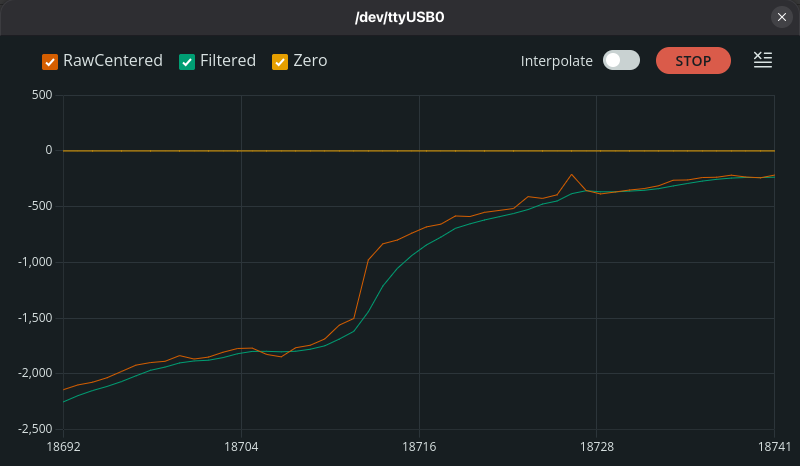
\includegraphics[width=\linewidth]{centered_filter.png}\caption{Centred input, filtered output and zero reference.}\end{subfigure}
\caption{Serial plotting during development on 13 October 2026. The uncalibrated ADC plots support qualitative signal conditioning observations. Axes do not establish physical time, clinical accuracy or a quantified before and after noise reduction.}\label{fig:adc}
\end{figure}

\begin{figure}[htbp]\centering
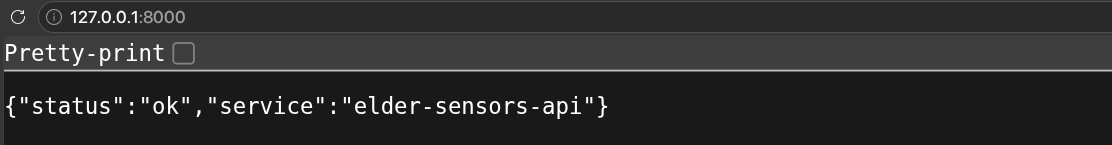
\includegraphics[width=\textwidth]{api_health.png}
\vspace{5mm}
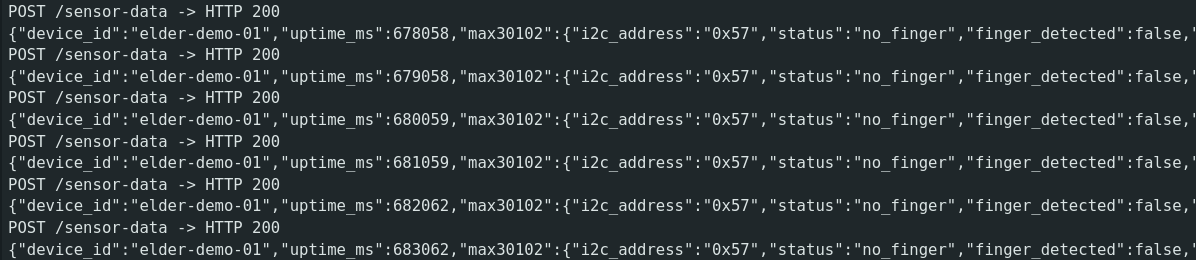
\includegraphics[width=\textwidth]{post_200_no_finger.png}
\caption{Local API availability and successful historical uploads on 13 October 2026. The old \code{/sensor-data} route returns HTTP 200 while the optical module reports \code{no_finger}. Successful transport does not establish measurement validity, persistent storage or the final versioned API.}\label{fig:http-history}
\end{figure}

\begin{figure}[htbp]\centering
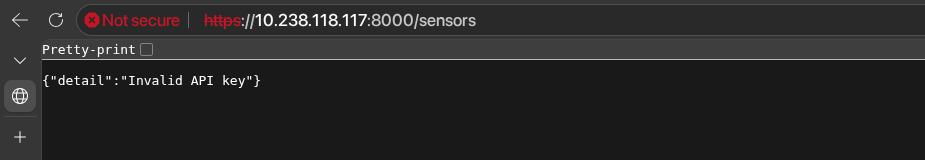
\includegraphics[width=\textwidth]{api_rejection.png}
\caption{Historical authentication rejection on 15 October 2026. The browser reports an invalid API key and also marks the connection insecure. This establishes a negative authentication path for that version; it is not evidence of trusted HTTPS or the current account based contract.}\label{fig:auth-history}
\end{figure}
\FloatBarrier
\clearpage
\section{Project team and development history}
\label{app:contribution}
The team roster identifies the academic submission. Repository chronology provides the technical change record; commit metadata is not used to infer a division of personal responsibilities or an individual contribution multiplier.

\begin{tabularx}{\textwidth}{@{}Y P{35mm}@{}}\toprule
Team member & Student ID\\\midrule
Nathan Ratichon & 2362789\\
Guannan Ge & 2364229\\
Jose Manuel Cortes Ceron & 2686162\\
Cheng Zhang & 2361292\\\bottomrule
\end{tabularx}

The tutor is Matilda Isaac. The names and IDs are reproduced as supplied by the team and are maintained in \path{metadata.tex}.

\begin{tabularx}{\textwidth}{@{}P{22mm}P{26mm}Y@{}}\toprule
Date & Commit & Recorded subject\\\midrule
25 Oct 2026 & \texttt{27a72d4} & Initial commit\\
25 Oct 2026 & \texttt{6757c0a} & upload files\\
25 Oct 2026 & \texttt{7e6c494} & upload csv files and data for ML part\\
26 Oct 2026 & \texttt{5c650c1} & update: mayor fixes\\\bottomrule
\end{tabularx}

The recorded Git identity is Jos\'e Manuel Cortes Cer\'on. The four commits establish the baseline chronology. The Android interface campaign and this report revision also include local working-tree changes, identified by the release input hashes rather than represented as additional commits. This preserves the distinction between committed history, supplied documentation and the exact built artefact.

\clearpage
\section{Demonstration protocol and evaluation boundaries}
\label{app:acceptance}
The demonstration separates three observable layers: native care navigation, synthetic server evaluation and the physical bench assembly. This structure prevents a successful result in one layer from being used as evidence for a different layer.

\begin{enumerate}
\item Identify APK 1.0.0/code 13 and its hash. Open the application on the Samsung and show the four-step account setup, explicit role selection, password visibility control and fixed primary action. The 709-check campaign records these interface behaviours, including registration text at 200\%.
\item Show role-specific navigation and grouped Settings. The caregiver has no wearable connection control; the connection page is inside authenticated Settings. The adult's source-defined wearable guide separates preparation, pairing, selection and recent-sample verification.
\item Run fixed Normal, Warning and Critical fixtures through the authenticated classification API. Display the response class, model score and synthetic source separately from the care interface. Readings and rule episodes use their own storage endpoints.
\item Exercise a sustained rule condition with three eligible samples, inspect the stored episode and compare the two caregivers' private inboxes. The recorded HTTPS fixture establishes fanout and independent review at the server boundary.
\item Retry a sample after a lost response and compare its stored identity. Show invalid or missing inputs producing rejection or an unknown state. The backend comparison and policy tests establish these properties without assigning handset delivery latency to them.
\item Present the physical assembly in Figure~\ref{fig:hardware-photo}, the source architecture and the recorded diagnostic aggregate. Explain which result comes from an image, a serial observation, a server test or a native interface check.
\end{enumerate}

\begin{table}[H]\small
\caption{Evaluation domains and the evidence supporting each claim.}\label{tab:acceptance}
\begin{tabularx}{\textwidth}{@{}P{34mm}Y P{37mm}@{}}\toprule
Domain & Recorded evidence and interpretation & Assessment relationship\\\midrule
Android interface & Installed code 13; 709 native checks; registration at text scale 2.0; role and Settings navigation & Mobile functionality and programming\\
Classification & Two trained models, held out matrices and authenticated server inference; scores describe synthetic classes & AI and REST\\
Persistence and alerts & 88 Python tests, 17 loopback HTTPS checks, 20 matched retry pairs and 20 episode trials & Data integration and testing\\
Hardware assembly & Original team photograph and 25-message diagnostic aggregate; image and runtime observation have distinct scope & Architecture and demonstration\\
Development trace & Team roster, four baseline commits and input hashes for the local release & Configuration and documentation\\\bottomrule
\end{tabularx}
\end{table}

The care Activity presents readings, alerts and settings; the history endpoint and chart component are separate from its current navigation, and classification scores are exposed by the server interface. The measured results concern these explicit system boundaries. They establish neither clinical efficacy nor a medical safety certification, and they do not turn a synthetic class score into a disease probability.

\clearpage
\subsection{Observed USB system execution: 30 October 2026}
\label{app:usb-run}
The current bench campaign uses real Bluetooth Classic SPP acquisition and real HTTPS requests from production Java and resources in an isolated Android application ID, \code{org.caremonitor.reportqa}. Its permissions and services come from the production manifest. A separate SQLite deployment on PC loopback port 19444 uses the existing trusted CA; adb reverse carries its HTTPS connection. Production accounts, the main application data and the laptop's Wi-Fi/VPN are preserved. The main installed application's separate USB deployment remains at port 19443.

The campaign creates controlled adult and caregiver accounts with fictional names, verifies that an unapproved caregiver sees no adult, requests a link and approves it, receives the physical wearable stream and checks the upload queue against retained server records. It then renders the native adult/caregiver pages using actual HTTPS results. These captures are not in-memory preview fixtures. Saved learning exercises explicitly use synthetic CSV examples. The temporary package is removed at the end, including its credentials and installation key; no default credentials are distributed.\cite{systemrun}

\begin{table}[H]\small
\caption{Recorded end-to-end observation boundaries. The first sample checkpoint precedes the later capture and database checkpoints, so their cumulative counts differ.}\label{tab:usb-observation}
\begin{tabularx}{\textwidth}{@{}P{38mm}Y@{}}\toprule
Observation & Evidence and meaning\\\midrule
Phone and software & Samsung S22 SM-S901E / Android 13, code 20 production Java/resources in the isolated report package. Its full input hash map is retained; the production APK installation has a separate hash and readonly client check.\\
Physical transport & 67 received samples at the first checkpoint in the measured campaign; both GY906 and MPU6050 reported online. The server later retained 76 device readings and the outbox reached zero pending.\\
Optical validity & Contact was supplied for a bench check. Reported optical status and validity flags are retained together: warming/invalid states are not presented as valid physiological readings. No accuracy or clinical population study is inferred.\\
Installed firmware & The installed image still reports legacy microphone/light fields. These do not establish connected modules. The corrected three-sensor source compiled without being flashed.\\
Role and AI execution & Approved caregiver reads the adult's retained history. Three synthetic learning exercises are saved through the real API and reviewed under both roles. Device temperature is not sent to the body-temperature model.\\
Capture campaign & \USBCaptureRecords{} device readings retained; representative record \USBRecordId{} with stable sample ID below. The device screen uses UTC+8 and may show 31 October while the UTC log remains 30 October.\\\bottomrule
\end{tabularx}
\end{table}

\begin{figure}[H]\centering
\resizebox{\linewidth}{!}{%
\begin{tikzpicture}[font=\sffamily\small]
\node[archbox,text width=3.05cm,minimum height=2.25cm] (board) at (1.75,0) {\textbf{1 / Physical ESP32}\\MAX / GY906 / MPU6050\\Validity flags + uptime\\Authenticated SPP NDJSON};
\node[archbox,text width=3.05cm,minimum height=2.25cm] (app) at (5.75,0) {\textbf{2 / Android relay}\\Timestamp + stable sample ID\\Encrypted outbox\\HTTPS POST /readings};
\node[archbox,text width=3.05cm,minimum height=2.25cm] (db) at (9.75,0) {\textbf{3 / FastAPI + SQLite}\\Validate and commit\\Retained record ID\\\USBRecordId{}};
\node[archbox,text width=3.05cm,minimum height=2.25cm] (ui) at (13.75,0) {\textbf{4 / Native views}\\GET overview + history\\Adult's selected resource\\Surface chart + reading details};
\draw[archflow] (board)--(app);\draw[archflow] (app)--(db);\draw[archflow] (db)--(ui);
\node[archnote,align=center,text width=14.8cm,anchor=north] at (7.75,-1.75)
 {Representative stable sample ID: \texttt{\USBSampleId}\\Captured at \texttt{\USBRecordTimestamp}. Source: device\_diagnostic.\\The chart aggregates the short bench interval; it is not a fabricated day-long waveform or a one-pixel-per-record trace.};
\end{tikzpicture}}
\caption{Representative sensor-to-API-to-mobile evidence chain from the controlled capture campaign. The server record and queue confirmation establish persistence; native views are fetched for that account and interval. A screenshot alone does not identify every aggregate contributor.}\label{fig:physical-trace}
\end{figure}

\subsection{Measured mobile response and native notification delivery}
Thirty S22 overview requests are timed from Android dispatch through parsed HTTPS response. Notification trials start at dispatch of a controlled synthetic confirmed SOS and end when NotificationManager exposes a new native care notification for the approved caregiver. Trials are seven seconds apart; each has a ten-second observation window. The two roles share one physical handset sequentially; the caregiver's foreground connection is active during delivery measurement. This is not a two-handset, locked-screen, audible-alarm or human-response experiment.

\begin{table}[H]\small
\caption{S22 USB measurements, in milliseconds, using linear-interpolated percentiles. Notification latency is conditional on successful posting; failed trials remain in the delivery denominator.}\label{tab:usb-latency}
\begin{tabularx}{\textwidth}{@{}Yrrrr@{}}\toprule
Operation / revision & N & Mean & p50 & p95\\\midrule
Overview HTTPS round trip, before & 30 & 57.80 & 71.19 & 75.69\\
Overview HTTPS round trip, final & 30 & 58.11 & 71.08 & 77.04\\
Native posting, before: 21/30; 9 timeouts & 21 & 546.51 & 559.35 & 977.38\\
Native posting, final: 30/30; 0 timeouts & 30 & 636.36 & 662.45 & 1094.37\\\bottomrule
\end{tabularx}
\end{table}

The first campaign exposed the S22's 25-notification package limit: Android rejected further native cards after the tray accumulated earlier cards and connection notifications. The original smoke runner completed but its nine recorded timeouts fail the strict delivery criterion; they have not been removed from the baseline. NotificationWindow now bounds event cards to twelve, including those scheduled earlier in the same batch. Evicting a native card neither acknowledges nor deletes its durable inbox item or alert. Two subsequent thirty-trial campaigns posted every requested notification within the observation window. The improvement is delivery completeness under this quota condition, not reduced successful-posting latency.\cite{systemrun}

The final source also translates newly generated and recognised historical system event defaults into English without changing user-authored text or rewriting encrypted historical records. A later capture pass records that presentation correction. Original timing arrays retain their own run identity and are not relabelled as newly measured values.

\newcommand{\SystemScreenPair}[5]{%
\begin{figure}[H]\centering
\begin{subfigure}[t]{.46\textwidth}\centering
\includegraphics[width=\linewidth,height=.65\textheight,keepaspectratio]{system/#1}
\caption{#2}
\end{subfigure}\hfill
\begin{subfigure}[t]{.46\textwidth}\centering
\includegraphics[width=\linewidth,height=.65\textheight,keepaspectratio]{system/#3}
\caption{#4}
\end{subfigure}
\caption{#5}
\end{figure}}

\clearpage
\subsection{Older adult: live acquisition and understandable readings}
\SystemScreenPair{elder_live_home_bottom.png}{Current thermal and movement cards; retired light card absent.}{elder_device_bottom.png}{Authenticated reception, server confirmation and zero pending uploads.}{Native S22 adult views during the real USB/SPP capture run. These controlled-account screens retain sensor validity and show live relay state. Counts continue increasing while pages are captured; they are checkpoints rather than a fixed total. The capture's complete hashes and original filenames are retained.}

\clearpage
\subsection{Older adult: stored history and separate learning results}
\SystemScreenPair{elder_history_top.png}{Surface history from retained device observations.}{elder_learning_bottom.png}{Saved synthetic classifications and model scores.}{Adult history and learning exercise results from real HTTPS responses. The short bench run contributes a small number of aggregate chart points. The synthetic confidence display is separate from the physical surface-temperature history; its score is not medical certainty.}

\clearpage
\subsection{Caregiver: selected person and reviewable notices}
\SystemScreenPair{caregiver_home_bottom.png}{Shared readings and the agreed care reminder.}{caregiver_alerts_top.png}{Controlled help notice awaiting this caregiver's review.}{Native approved-caregiver views from the isolated capture campaign. The help event is labelled test data, and acknowledgement is a human review action rather than proof that an emergency response occurred. Names identify fictional test accounts; the device observations originate from the bench assembly.}

\clearpage
\subsection{Caregiver: authorised history and saved synthetic confidence}
\SystemScreenPair{caregiver_history_top.png}{History explicitly names the selected adult.}{caregiver_learning_bottom.png}{Read-only access to that adult's retained exercises.}{Caregiver access is acquired through an invitation, request and adult approval before these real API-backed views are captured. Historical charts and saved class/confidence are demonstrated on the handset, while location/audio permissions remain separate opt-ins.}

\clearpage
\section{Current system architecture atlas}
\label{app:system-atlas}
This atlas documents the user-specified three-sensor wearable and the canonical Android/FastAPI implementation. The removed microphone and light module are absent from the current wiring topology. Legacy JSON fields and a BLE transport client may remain compatible software contracts; they do not identify additional installed hardware. The earlier assembly photograph is retained with its date rather than altered to resemble a new photograph.

\textbf{Reading the figures.} Solid teal arrows identify implemented transfers or dependencies. Dashed arrows are responses or class dependencies where stated. Amber panels identify requested behaviour requiring further implementation or validation. A line documents a technical responsibility; it does not imply that every deployment or clinical outcome has been tested.

\WearablePurposeFigure
\clearpage
\subsection{Electrical connections and pin ownership}
\WearableWiringFigure
\clearpage
\subsection{Transport protocols and wire formats}
\ProtocolStackFigure
\clearpage
\subsection{Actors and approval boundaries}
\ActorsDiagram
\clearpage
\subsection{Mobile navigation and task flow}
\MobileFlowDiagram
\clearpage
\subsection{Selected production classes}
\MobileClassDiagram
\clearpage
\subsection{Permissions and optional phone capabilities}
\PermissionsFigure
\clearpage
\subsection{Server components and source separation}
\ServerArchitectureDiagram
\clearpage
\subsection{Server classes and function-based services}
\ServerClassDiagram
\clearpage
\subsection{Persistent data domains}
\DatabaseDiagram
\clearpage
\subsection{Authentication and encryption boundaries}
\SecurityProtocolDiagram
\clearpage
\subsection{Capability interpretation for the current assembly}
\begin{table}[H]\small
\caption{Measured inputs, implemented behaviour and requested extensions. Clinical thresholds are not specified by this diagram set.}\label{tab:current-capabilities}
\begin{tabularx}{\textwidth}{@{}P{29mm}P{47mm}Y@{}}\toprule
Area & Available input / behaviour & Claim boundary or next implementation\\\midrule
Pulse and oxygen & MAX30102 optical estimates with contact, calculation and validity flags & Estimates need stable optical coupling. Invalid values stay unavailable; no clinical accuracy claim follows from sensor presence.\\
Surface / ambient & MLX90614 object and local sensor temperature & Explain both channels. Ambient at the sensor is not a certified room measurement; surface is not core temperature. Current extreme-temperature rule demonstrations use synthetic input.\\
Wear detection & Optical-contact and sample-quality indicators & No contact can prompt a placement/connection check. No readings can also mean motion, disconnection or a fault; it is not a definitive not-worn state.\\
Walking / falling & MPU6050 acceleration and angular velocity & Current acquisition provides motion data. Step counting, real-time fall classification and a local fallback alarm are not implemented by this source. SisFall is an independent offline experiment.\\
Location & Phone GPS/location with consent, accuracy and expiry & Adult permission and server consent are required; caregivers see only approved shared data. Network and OS conditions affect availability.\\
Help and sound & Confirmed help event, durable private inbox and Android notification channel & Native posting can be measured. Audibility, hearing the alarm, response and emergency-service contact are different outcomes.\\
Buzzer fallback & GPIO25 output configured LOW & A fallback needs detection logic, an appropriate driver and independent power. No autonomous fall-triggered tone is established.\\
Hydration & Agreed hydration reminder in the care plan & These modules do not measure dehydration. A reminder is not a physiological assessment.\\
Energy & Phone handles GPS, uploads, storage and notifications & Offloading simplifies the wearable. Larger battery capacity alone does not establish longer runtime; current draw and endurance require measurement.\\\bottomrule
\end{tabularx}
\end{table}

The component roles are checked against manufacturer descriptions for MAX30102 and MLX90614, and against the actual register acquisition in the firmware.\cite{maxdatasheet,mlxproduct} Electrical labels describe breakout modules, not direct wiring to bare IC dies. The carrier's physical header order and supply selector must be checked on the actual KEYES revision; this source-derived map does not replace that inspection.

\end{document}
